\documentclass{article}
\usepackage[utf8]{inputenc}

\title{detectorhandins}
\author{Daniel S. Nielsen, Rosanna Ignazzi, \\Étienne Bourbeau, Fabian A.J. Thiele}
\date{October 2018}
\usepackage{siunitx} % SI units
\usepackage{amsmath} % equations
\usepackage{tabularx}
\usepackage{tikz}
\usepackage{hyperref}
\usepackage{ifthen}
\usepackage[T1]{fontenc} % proper underscores etc.
\usepackage{subcaption} % replace subfloat with subfigure env.
\usepackage{float}
\usepackage{todonotes}
\usepackage{placeins}
\setlength{\parskip}{.8em} % add some space btwn paragraphs


\sisetup{per-mode=fraction}

\begin{document}
	% === Front matter ====================================================

	%\frontmatter
	\maketitle
	
	\tableofcontents
	
	%\listoffigures
	
	%\listoftables
	
	%\lstlistoflistings
	
	\cleardoublepage
	
\begin{abstract}

In order to gain a better understanding of proportional gas detectors and their operation, in this experiment we describe how to build one with householding items, in particular with a cider can as the tube to be filled with gas (cathode) and a common wire from a low voltage cable (anode), and one with more advance items.
To read out the charge collected in the wire from the gas ionisation from two particle sources, Fe-55 and Am-241, the detector is connected to a preamplifier and a computer with a Multi-Channel Analyser. With the collected charge measurements we can compare the gas multiplication factor measured with the one predicted by the analysis setup and by the experimental environment. The measured values are within $1\sigma$ of the predicted values. 
A measurement of the energy spectra for Am and Fe are also possible with the experimental setup and they are usefult to identify the energy peaks for different interactions.

\end{abstract}

%\clearpage
	
	\clearpage
	\section*{Introduction}  \label{sec:Introduction}
\addcontentsline{toc}{section}{\protect\numberline{}Introduction}

	
	
	
	
	% === Main matter =====================================================

        % Report structure reflects the structure laid out in todo.txt
	
	% --- Chapter 1: Background -----------------------------------------------
	
	\cleardoublepage

        \clearpage
	\section{Gas Detector construction}
\label{sec:construction}

For the physical measurements of the elements of the detectors, either a caliper or a micrometer were used. Their precisions lead to systematic uncertainties of $\SI{0.05}{\milli\meter}$ and $\SI{0.005}{\milli\meter}$, respectively.

\subsection{Cider can}
We have been handed a start-up kit consisting of one empty $\SI{500}{\milli\liter}$
cider can, two Plexiglas endcaps, two Teflon pipes, one nylon screw and nut,
brass pipes and a high voltage (HV) connector with a small exterior connector for
grounding the outside of the can.

\begin{table*}[htb]%
% \begin{maybeleft}%
  \begin{tabularx}{\linewidth}{p{4cm}p{1.5cm}p{3cm}p{2cm}}
    \textbf{Element}       & \textbf{Symbol} & \textbf{Mean}            & \textbf{Tool used} \\ \hline
    Can diameter           & $D_{outer}$     & $65.82 \pm 0.22$~mm      & caliper            \\
    Can wall thickness     & $\tau$          & $\SI{105}{\micro\meter}$ & micrometer         \\
    Plastic tube diameter  & $d_{t}$         & $5.97 \pm 0.05$~mm       & caliper            \\
    Brass tube diameter    & $d_{brass}$     & $1.0$~mm                 & caliper            \\
    Nylon screw diameter   & $d_{screw}$     & $7.78 \pm 0.04$~mm       & caliper            \\
    HV connector diameter  & $d_{HV}$        & $9.37$~mm                & caliper            \\
    Anode wire diameter    & $d_{wire}$      & $\SI{50}{\micro\meter}$  & micrometer         \\ \hline
  \end{tabularx}
  \caption{Measurements of the cider can experiment setup components. Measurements without uncertainties were only measured once and are dominated by the systematic uncertainties of the measurement tools.}
  \label{Tab:cidercan_sizes}
% \end{maybeleft}%
\end{table*}

The process started with the preparation of the cider can which included cutting
away the top part of the can, removing the inner coating with a drill equipped with a
metal brush on top, drilling two holes in the bottom: one in the middle of the
endcap for the nylon screw and one slightly offset from the center for the
gas exchange system (of $d = \SI{8.0}{\milli\meter}$ and $d =
\SI{6.0}{\milli\meter}$). The second step consisted in drilling the necessary
holes in the Plexiglas endcaps (which already have a groove for the can
extremities to be fitted in): one hole for the gas Teflon pipe in the back
endcap and one for the front endcap, as well as a hole for the HV connector in the
front endcap (the diameters are $d = \SI{6.0}{\milli\meter}$ and $d =
\SI{9.5}{\milli\meter}$ respectively). Finally a small hole of $d =
\SI{1.0}{\milli\meter}$ was drilled in the Teflon screw, in order to insert the
brass pipe in there at a later point. The brass tubes were cut and flattened
with sand paper, to remove the part that was squeezed due to the cutting tool.

\begin{figure}[htb]
  \centering
  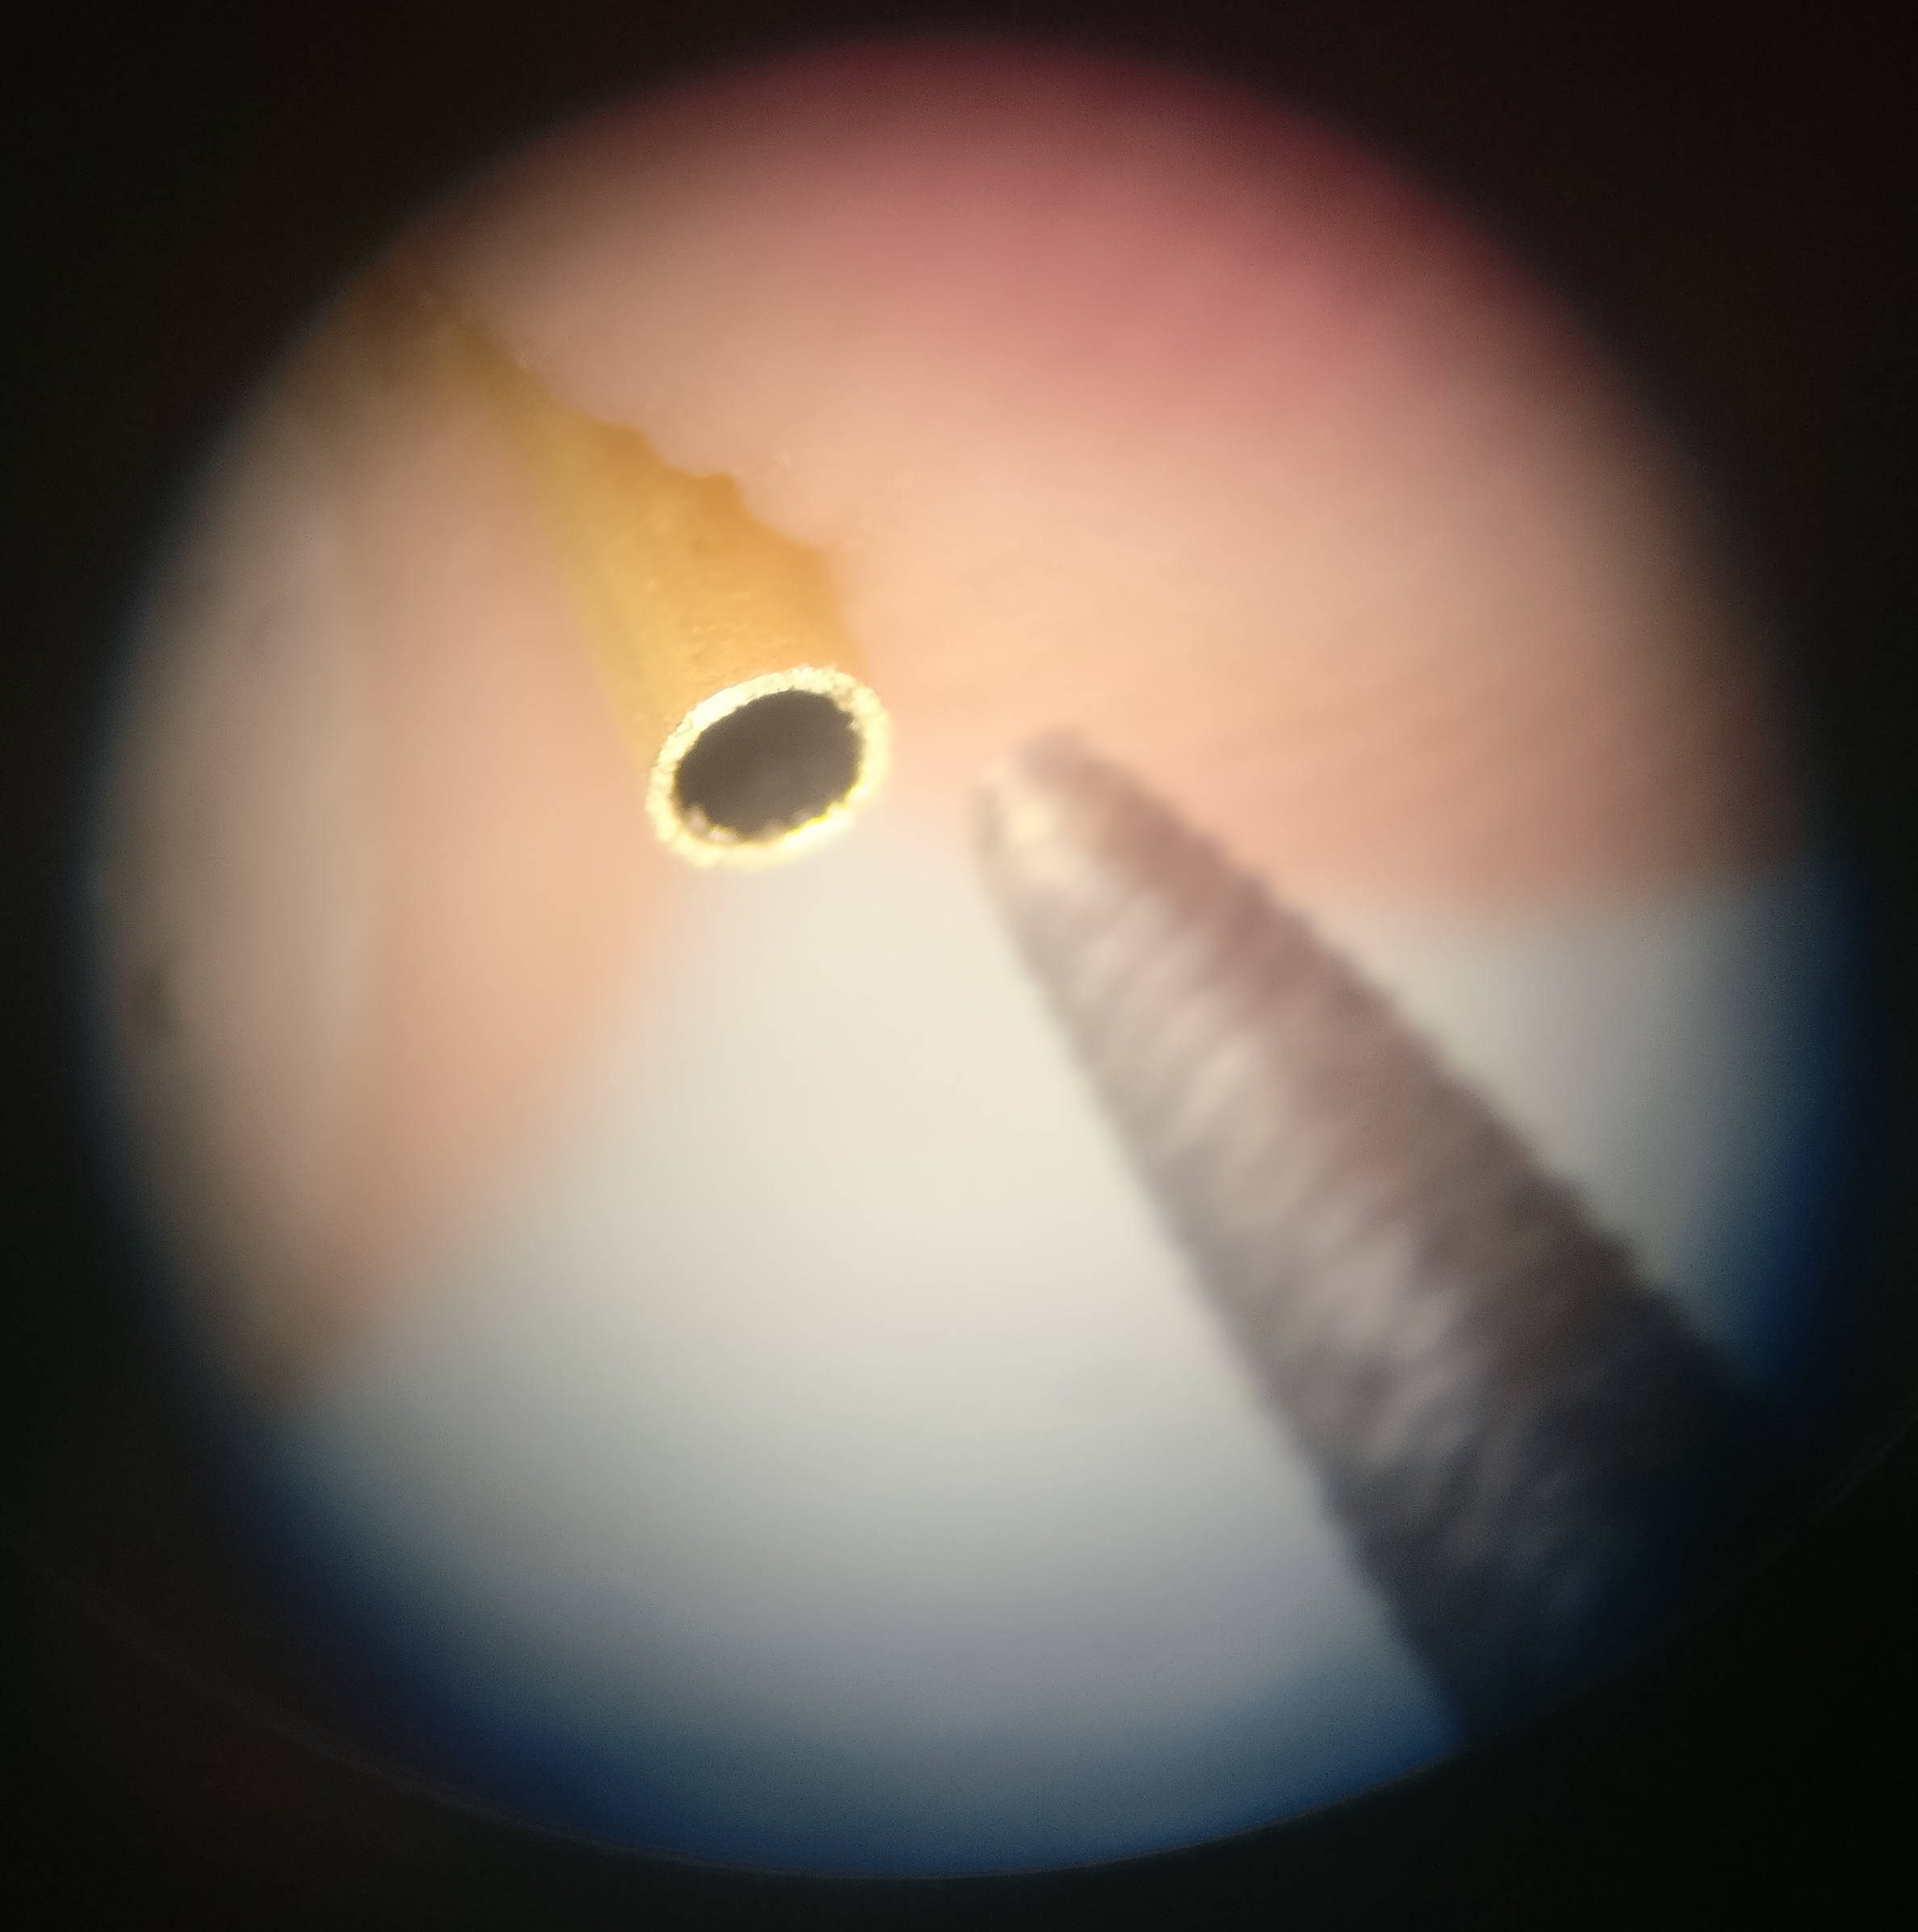
\includegraphics[width=0.5\textwidth]{./graphics/brass_file.jpg}
  \caption{Filing of the brass tube}
  \label{fig:brass_file}
\end{figure}


Once all the ingredients were ready, all the holes in the can and the edges of
the brass tube were filed and checked under a microscope (see Fig.~\ref{fig:brass_file}), in order to avoid
sharp edges. All the components were placed in an isopropanol (IPA) bath in a
sonicator, so all the skin oils and dirt were cleaned off, and all parts were
dried with $\mathrm{N}_2$ gas. At this point, the only element missing was the
anode wire, which was taken from a regular low voltage cable and carefully wiped
with a cloth dipped in IPA.


The assembly of the detector started with the fastening of the nylon screw and
bolt to the aluminium can, using the hole in the middle of the bottom of the
can. The longer of the two brass tubes was inserted in the nylon screw, and one
end of the anode wire was passed in the brass tube from the outside and pulled
until the other end of the can. On the other extremity of the anode wire, a
small nut was attached with a simple knot, in order to help keeping the anode
wire straight later on in the process. The free end of the wire was inserted in
the shorter brass tube and both were soldered to the HV connector, which
had been previously fastened to the front Plexiglas endcap (a small contact
has been placed between the HV connector and the outer glass, to later
use it for grounding the cathode). The front endcap was glued with epoxy to the
cider can and was left to dry for some time. The next step consisted in
straightening out the anode wire inside the can by pulling it slowly out of the
can from the bottom. The wire has to be quite straight in order to avoid dips,
where the charge could concentrate and obscure the measurement. To reach an
optimal condition, a weight was carefully lowered to slowly apply tension.
When a satisfactory straightness was achieved, the wire was soldered to the
brass pipe and the rest cut off. The back endcap was glued to the cider can and
left to dry for some time.

The gas Teflon tubes were glued to the front and back endcap and a small
quantity of glue was applied around the HV connector, to ensure optimal
insulation.

Before moving on to the next step, a leakage test was performed, to check for
possible holes in the glue. The gas supply (in our case $\mathrm{P10}$) was
attached to one of the Teflon gas tubes and to a flowmeter, which measured a gas
flow of approximately \SI{25}{\milli\liter\per\minute} out of the tube. When
moving the flowmeter to the other end of the can detector, the gas flow measured
was between \SI{2}{\milli\liter\per\minute} to \SI{4}{\milli\liter\per\minute}, which meant that an extra layer
of glue had to be applied to the outside and the endcaps and to the tube
connections, to cover potential leaks. After this adjustment, the gas
flow was measured again and the gas flow injected in the detector was
\SI{18.3}{\milli\liter\per\minute}, while the outgoing gas flow was of
\SI{17.6}{\milli\liter\per\minute}. This was determined to be sufficient for the
purpose of the experiment.

The last step consisted in removing some of the coating from the outside of the cider can with sand paper, and connecting the grounding pin previously attached
to the HV connector to the bare aluminium of the can with copper tape. This tape would later be grounded to the cathode to create the electric field inside the can. The
connection was checked with a multimeter, where it was asserted, that there is no connection between the cathode can and the anode wire.

\subsection{Copper Tube}

\label{sec:copper_construction}
A more sophisticated detector made out of copper was built after the more rudimentary one. In this case, the gas proportional chamber detector was made out of a machined copper tube. The end caps were made out of two Teflon plugs, brass tubes were again used as electric field protector, and a finer, copper beryllium wire was selected as the anode material. The material also included smaller Teflon pipes for the gas inlets, the same HV connector and the same grounding pin as in the cider can assembly. Fig.~\ref{fig:copper_parts} shows all parts of the assembly.

In order to ensure that the X-ray emission from the source would be able to penetrate the thicker walls of the copper tube, a hole of $5$ mm was drilled in the copper tube, approximately in the middle of the pipe. The Teflon plugs were filed down in order to match the inner radius of the copper pipe and the pre-existing holes for the gas supply tubes. The holes for the HV connector and brass tubes were adjusted to the appropriate sizes of the different components. Similarly to the previous detector, the brass pipe was sanded and filed at the edges to remove any sharp debris that would cause sparking.

All the parts were cleaned in an IPA bath and dried with N$_2$. The wire was soldered to the brass tube and to the HV connector and inserted carefully in the copper tube. This part of the procedure was much more delicate than in the previous assembly, given the tendency of the much thinner wire to curl on itself and break easily. The copper tube was glued with epoxy to the front Teflon plug. The wire was then passed into the second brass tube and in the back Teflon plug  The back plug was glued and the wire soldered to the brass tube.

\begin{figure}[htb]
  \centering
  \includegraphics[width=0.5\textwidth]{./graphics/copper_tube_parts.jpg}
  \caption{Cleaned parts of the copper tube assembly}
  \label{fig:copper_parts}
\end{figure}

Finally, the hole drilled for the target was covered by a small piece of metallic tape, held in place by epoxy glue to seal off the opening.

\subsubsection{Testing}

The copper tube detector was flushed and then filled with P10 gas and connected to the amplifier electronics in a similar fashion as the previous detector. Unfortunately, preliminary observations of the signal at the oscilloscope indicated a problem with the state of the detector, as no pulses appeared on the screen even in the presence of a radioactive source. Further investigation led us to realise that the HV connector became electrically shorted when leftover parts of the anode wire (the excess wire that was mistakenly not cut) came into contact with the outer part of the HV connector, as the end cap was inserted into the tube. This rendered the device inoperable. To perform the same measurements as in the cider can experiment and thus compare the two proportional gas detectors, we relied on measurements taken with a reference copper tube detector.
Results in Sec.~\ref{sec:spectraanalysis} have thus not been made with the instrument characterised in Tab.~\ref{Tab:coppercan_sizes}.

\begin{table}[htb]
	\begin{tabularx}{\linewidth}{p{4cm}rp{2cm}}
		\textbf{Element}                   & \textbf{Mean}~{[}mm{]} & \textbf{Tool used} \\ \hline
		Cu tube, length                    & $149.08 \pm 0.02$      & caliper            \\
		Cu tube, wall thickness            & $1.04 \pm 0.04$        & caliper            \\
		Cu tube, inner diameter            & $19.91 \pm 0.11$       & caliper            \\
		Cu tube, radiation hole            & $5.05 \pm 0.03$        & caliper            \\
		HV frontend, total length          & $36.79 \pm 0.04$       & caliper            \\
		HV frontend, top part length       & $15.90 \pm 0.04$       & caliper            \\
		HV frontend, tube extremity radius & $19.85 \pm 0.01$       & caliper            \\
		backend, total length              & $14.97 \pm 0.07$       & caliper            \\
		backend, top part length           & $4.99 \pm 0.05$        & caliper            \\
		backend, tube extremity radius     & $19.87 \pm 0.01$       & caliper            \\
		Brass tube diameter                & $1.000$                & caliper            \\
		Anode wire thickness               & $0.025$                & micrometer         \\ \hline
	\end{tabularx}
\caption{Measurements of the copper pipe experiment setup components. Measurements without uncertainties were only measured once and are dominated by the systematic uncertainties of the measurement tools.}% The ends are made of Teflon.}
\label{Tab:coppercan_sizes}
\end{table}

\subsection{Aliminium tube}
For this experiment, additional measurements were performed with an aluminuium tube proportional counter detector. In this case, the aluminium detector was assembled by group 2. For the data with this detector, we have no physical parameters (with their uncertainties) or calibration measurements, and as such, the theoretical calculation of the charge multiplication is not possible.

% For the analysis, the spectra measurements made by the aluminium tube assembled by group 2 have been used. No physical, calibration, nor systematics measurements of their detector is available, and as such, all theoretical calculations are only made for the can detector.    % Fabian
        
	\clearpage
	\section{Experimental setup Cali\-bra\-ti\-on}

\subsection{Set-up}
\label{sec:calibration:set-up}
Before performing the source spectra measurements, the detector was connected to the HV power supply and to an amplifying circuit consisting of a \textit{preamplifier} and a \textit{coarse-gain amplifier}, shown on respectively in figure \ref{fig:preamp_photo} and \ref{fig:ampli_gene}. 

\begin{figure}[htb!]
  \begin{subfigure}[b]{0.45\textwidth}
    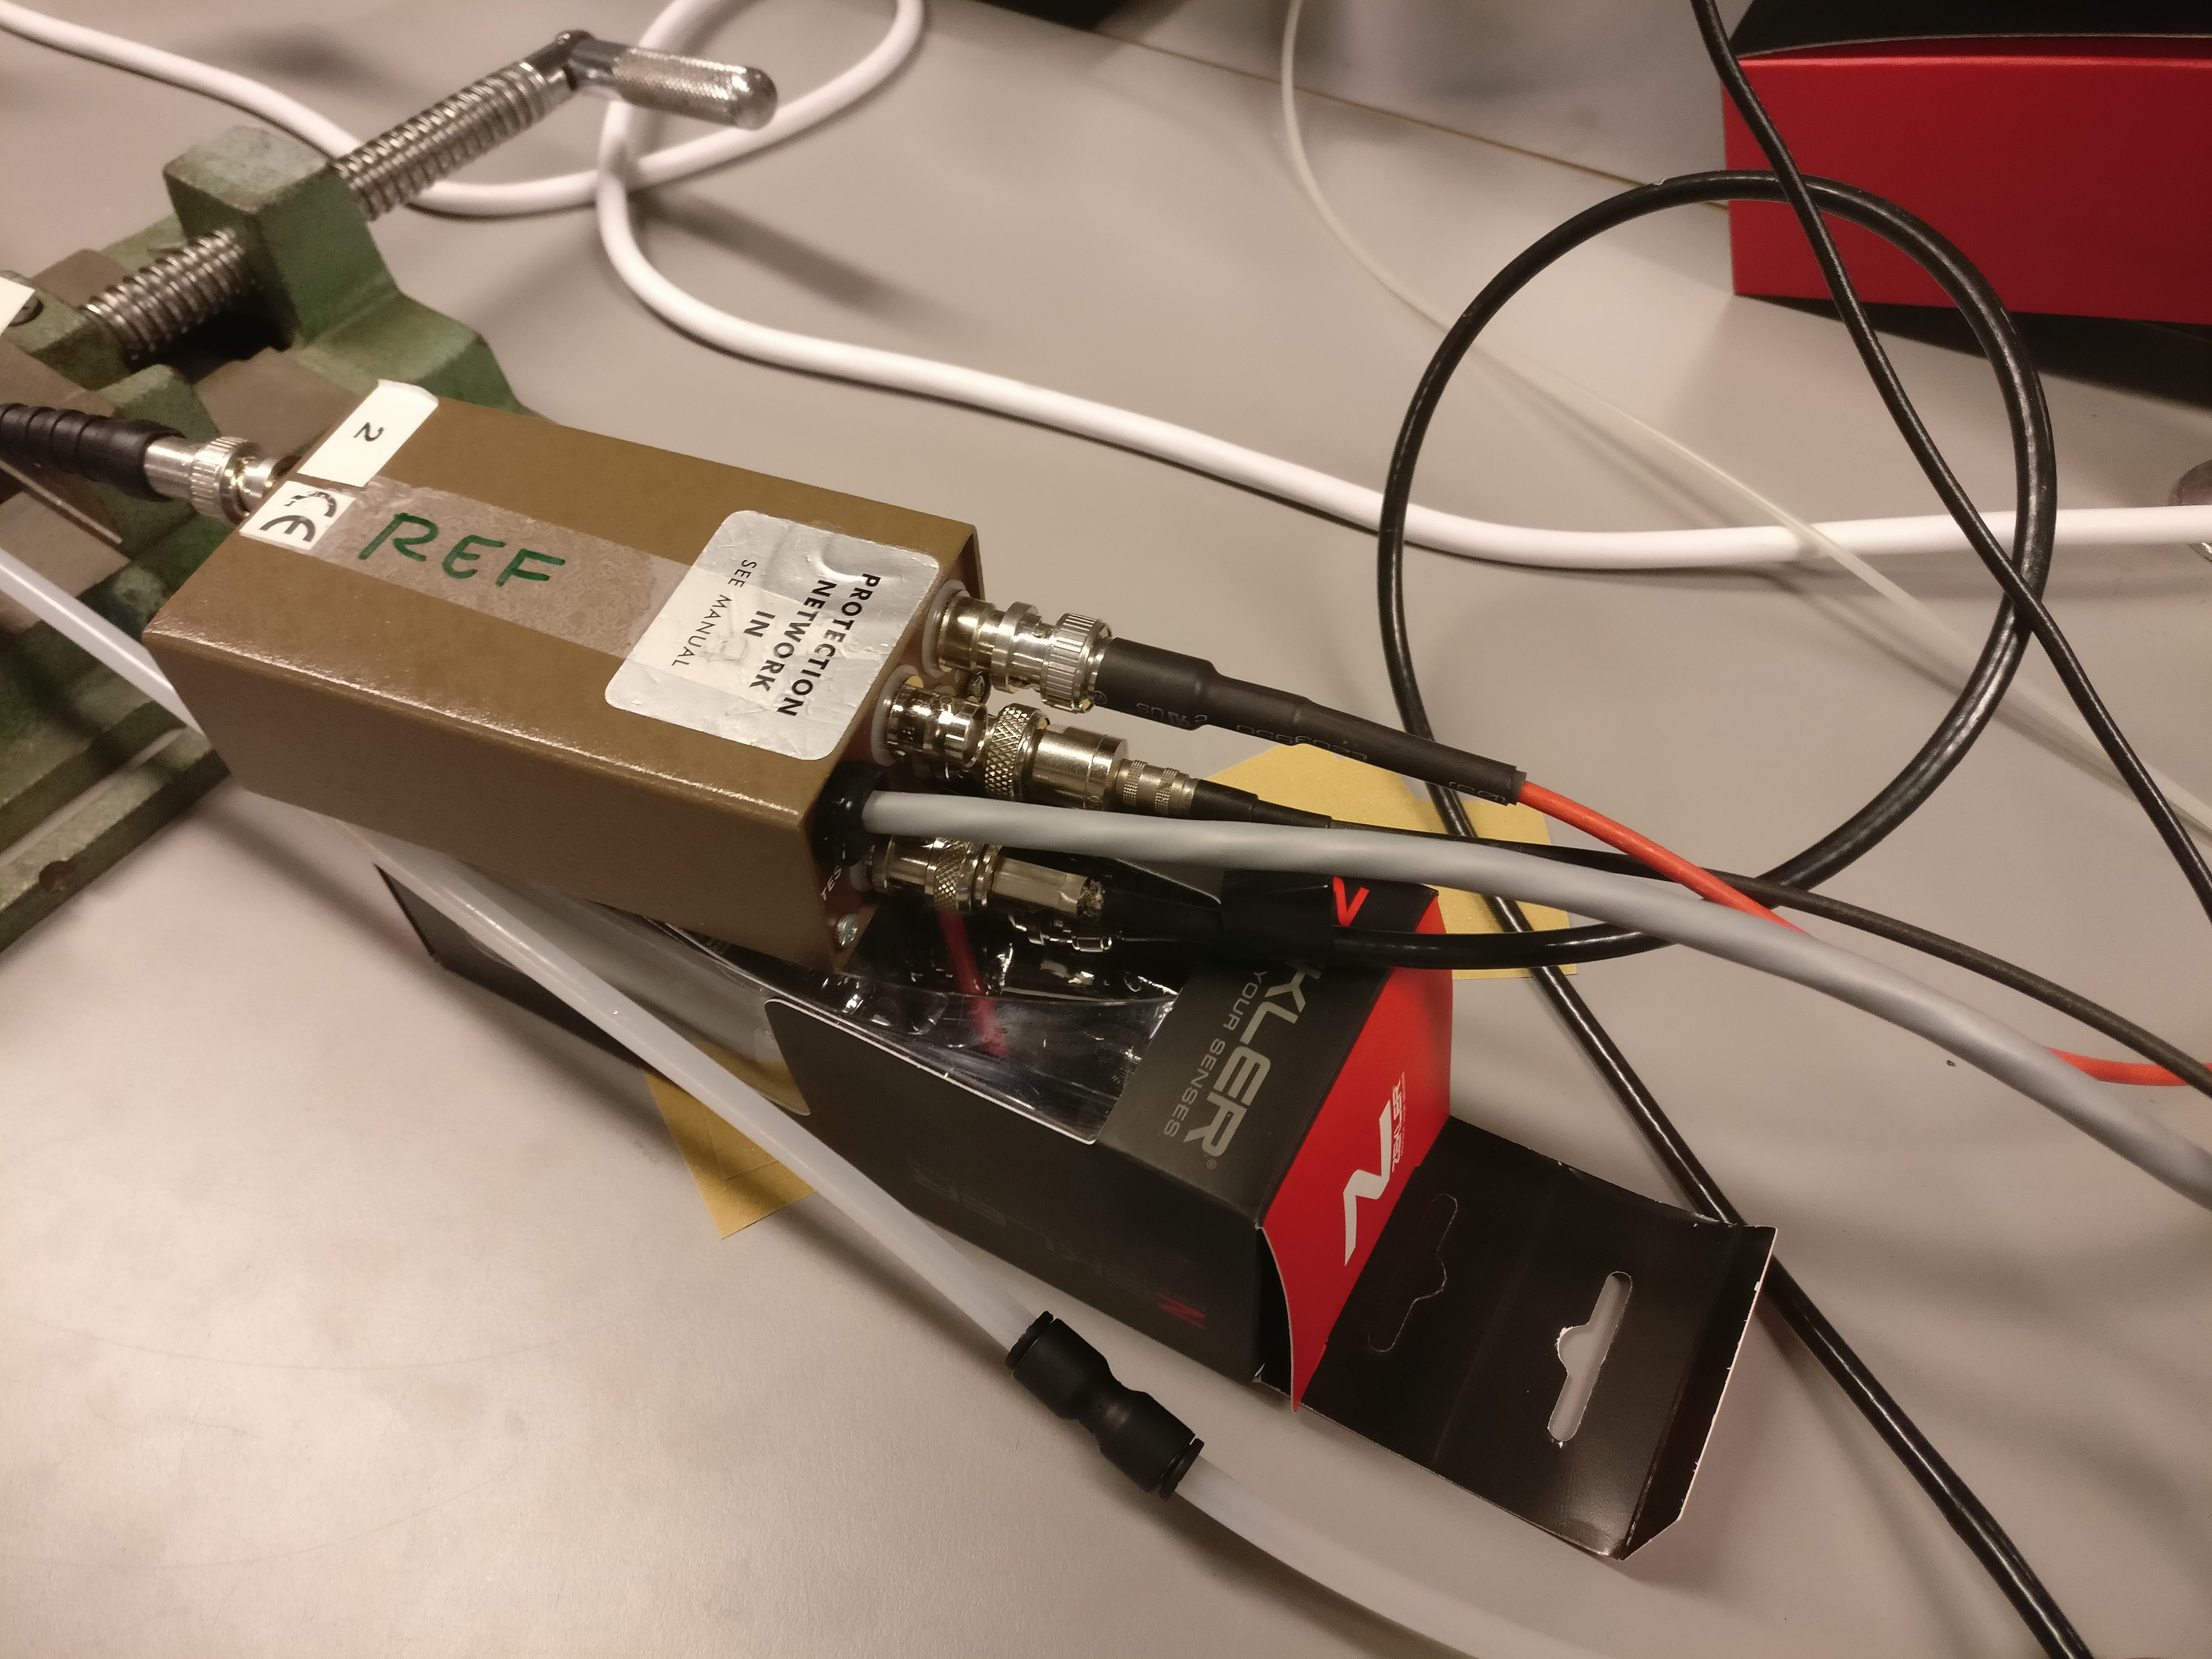
\includegraphics[width=\textwidth]{graphics/preamplifier.jpg}
    \caption{}
    \label{fig:preamp_photo}
  \end{subfigure}
  ~
  \begin{subfigure}[b]{0.5\textwidth}
    \includegraphics[width=\textwidth]{graphics/amplifier_photo.jpg}
    \caption{}
    \label{fig:ampli_gene}
  \end{subfigure}
  \caption{a) Photograph of the preamplifier unit. b) Photograph of the pulse generator used to inject pulses into the preamplifier, and the coarse gain amplifier used in front of the MCA.}
\end{figure}

Both system contribute to increase the overall number of signal electrons collected per avalanche occurring in the drift chamber. The overall gain in signal, between the drift chamber electrode and the final Multi-Channel Analyser (MCA) reading out data, is given by equation \ref{eq:gain_system}.

\begin{equation}
  \label{eq:gain_system}
  Q_{MCA} = Q_{drift}\cdot G_{pre}\cdot G_{coarse}
\end{equation}


\subsection{Calibration of the pre\--amp\-li\-fi\-er gain}
 Calibrated pulses of various intensities were injected into the electronics, and the output was displayed onto an oscilloscope to evaluate the gain of the preamplifier, $G_{pre}$ and its uncertainty. Figure \ref{fig:preamp_gain} shows the result of this measurements, where the data was fitted to a line. Note that the slope of the line corresponds to 10 times the gain of the preamplifier: this is because the entire calibration measurement was performed at a nominal coarse gain of 10. This correction factor is accounted for when quoting the gain that is only due to the pre\--amplifier, $G_{pre} = 6.41 \pm 0.01$.

\begin{figure}[htb!]
  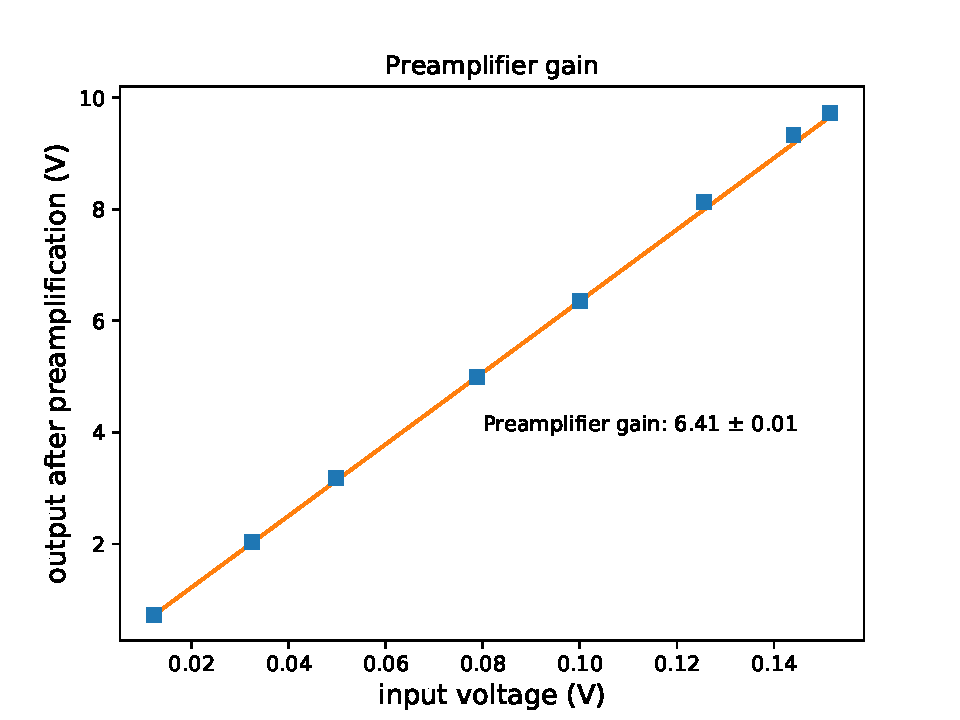
\includegraphics[scale=0.5,width=0.5\textwidth]{graphics/preamp_gain_calibration.pdf}
  \caption{Output voltage of pulses injected into the pre\--amplifier electronics. The quoted gain on the figure and the slope of the line differ by a factor of 10.}
  \label{fig:preamp_gain}
\end{figure}

In later sections of this report, it will be more useful to quote the preamplifier gain in units of $d.c/V$, as the later measurements have been done using the Multichannel analyser (MCA), and not of the oscilloscope. Figure \ref{fig:preamp_gain_mca} presents the preamplifier gain in these units. Once again, a correction factor of 10 is applied to remove the coarse gain value from the result.

\begin{figure}[htb!]
  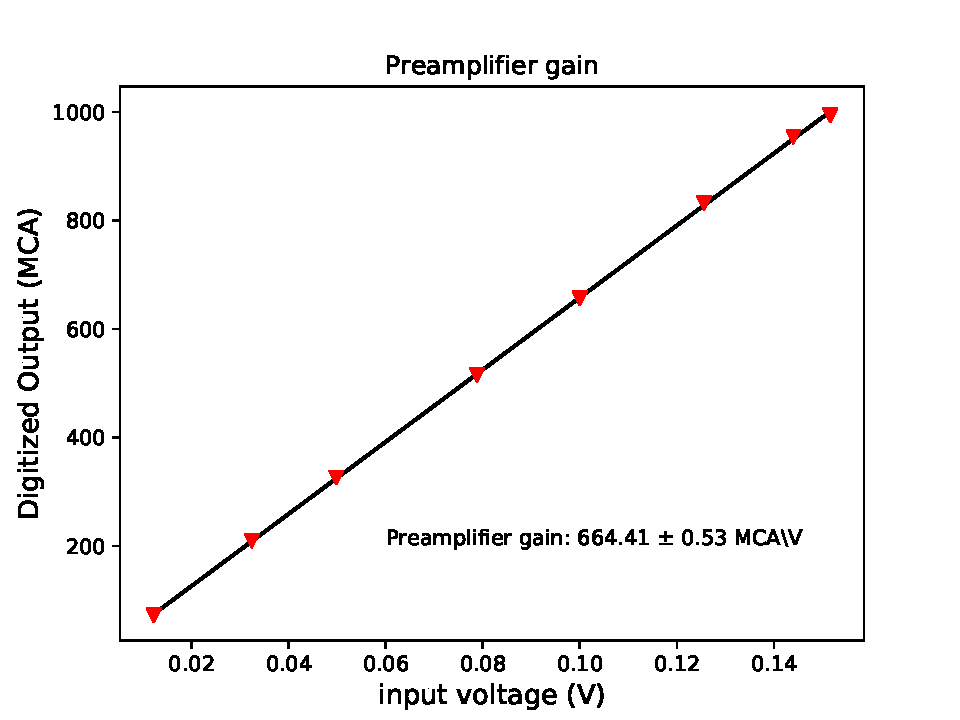
\includegraphics[scale=0.5,width=0.5\textwidth]{graphics/preamp_gain_calibration_plus_conversionfactor.pdf}
  \caption{Measurement of the preamplifier gain, in terms of digital counts taken from the Multi Channel Analyser (MCA) The quoted gain on the figure and the slope of the line differ by a factor of 10.}
  \label{fig:preamp_gain_mca}
\end{figure}


\subsection{Calibration of the coarse~gain amplifier}
\label{sec:coarse}
To estimate the uncertainty on the coarse gain amplifier, subsequent runs of Fe$^{55}$ and Am$^{241}$ spectra acquisitions were made at the same operating voltage, but different coarse gain settings. These measurements allowed us to measure the \textit{ratios of coarse gains} between subsequent settings of the amplifier knob, with corresponding uncertainties.

Figure \ref{fig:coarse_gain} shows the result of this analysis. Since the data acquired only allowed us to measured ratios of gain settings, the uncertainties of the absolute amplifier gain are simply assumed to scale with the default setting of 10, used in the previous calibration measurement. This means that for the purpose of error propagation, each coarse gain was defined with respect to the following rules

$$
G_{coarse} = \left\{
\begin{array}{ll} 
  10\cdot\Pi_{j>i}^{j\leq10}\frac{G_{j}}{G_{i}} & (i) \in [2,4] \\
  10 & i=10 \\
  10\cdot\Pi_{j>i}^{j\leq 100}\frac{G_{j}}{G_{i}} & i \in [20,40] 
\end{array}
\right.
$$

where $j$ is the higher level of a pair of coarse gain settings. Figure \ref{fig:coarse_gain} presents the various ratios of gain settings measured, using both the Fe$^{55}$ and Am$^{241}$ source. The red data point show the result of combining both results, which allows us to get better estimates of the gain ratio uncertainties.

\begin{figure}[htb!]
  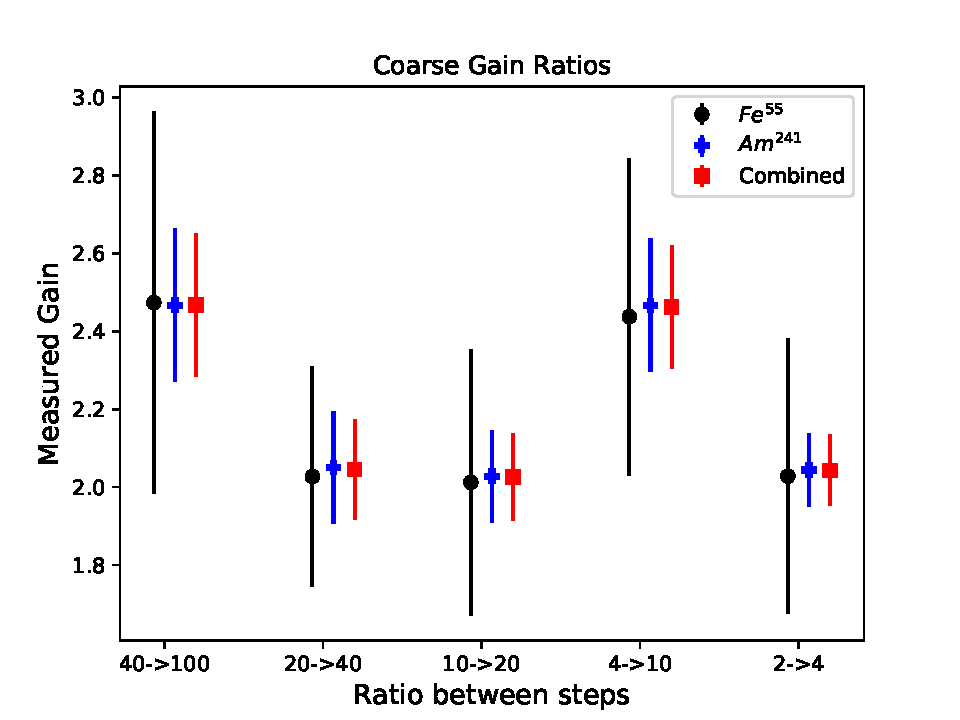
\includegraphics[width=0.5\textwidth]{graphics/coarse_gain_calibration.pdf}
  \caption{Determination of the coarse gain amplification uncertainties. Results are presented in the form of gain ratios between every adjacent setting of the coarse gain knob. The combined value and uncertainty on each measurement is shown by the red data points.}
  \label{fig:coarse_gain}
\end{figure}


As stated above, the use of gain ratio is useful for propagating the uncertainty on $G_{coarse}$, when considering the effect of systematics on the global yield of charge carrier in the drift chamber (see section \ref{sec:systematics}).
    % Etienne

	\clearpage
	\section{Energy scale calibration}
\label{sec:energy_scan}

\subsection{Resolution Scans}
\label{sec:resolution_scans}
As the signal from the detector is rather weak, the detector is connected to an
amplifying circuit as described in Sec.~\ref{sec:calibration:set-up}. However
there is a trade-off associated with this procedure as amplification also
applies to noise in the detector. In order to increase the signal strength the
voltage applied to the detector can be increased which in turn increases the
amount of signal electrons and leads to a stronger output signal. Along with
this comes though an increased probability for spontaneous discharges along
impurities and dirt remaining in the detector despite extensive cleaning
procedures as described in Sec.~\ref{sec:construction}.

As the two possibilities for varying the output signal strength are associated
with independent increases of noise and accordingly reduction of resolution we
are performing resolution scans for the two samples we are interested in
measuring: Americium and Iron.

In order to reliably determine the resolution a Gaussian is fitted to the sample
peak previously identified in the MCA spectrum. We look
at the variable peak width divided by the peak position in order to determine
the resolution of our peak. For the peak width we are using the full-width
half-maximum (FWHM) value. As secondary decays will affect especially the lower
end of the decay Gaussian \todo[inline]{how are they called exactly? secondary seems
  wrong} shape we are defining regions of interest (ROI) in which the Gaussian
is fitted.

The spectra obtained for americium (Fig.~\ref{fig:scan:americium}) and iron
(Fig.~\ref{fig:scan:iron}) are presented in App.~\ref{app:resolution-scans} for different gains and voltages.
A Gaussian is fitted to the marked ROI (blue lines) and the obtained channel number as well as
full-width half-maximum (FWHM) in channels are denoted in each figure.

The obtained parameters from the fit are plotted in Figs.~\ref{fig:resolution:americium} and \ref{fig:resolution:iron} for americium and
iron respectively. The uncertainties are propagated from the fit. Additionally to the
total uncertainty on the FWHM, a \SI{10}{\percent} systematic
uncertainty was added due to the dependency on choosing the corresponding ROI.

\begin{figure}[htb]
  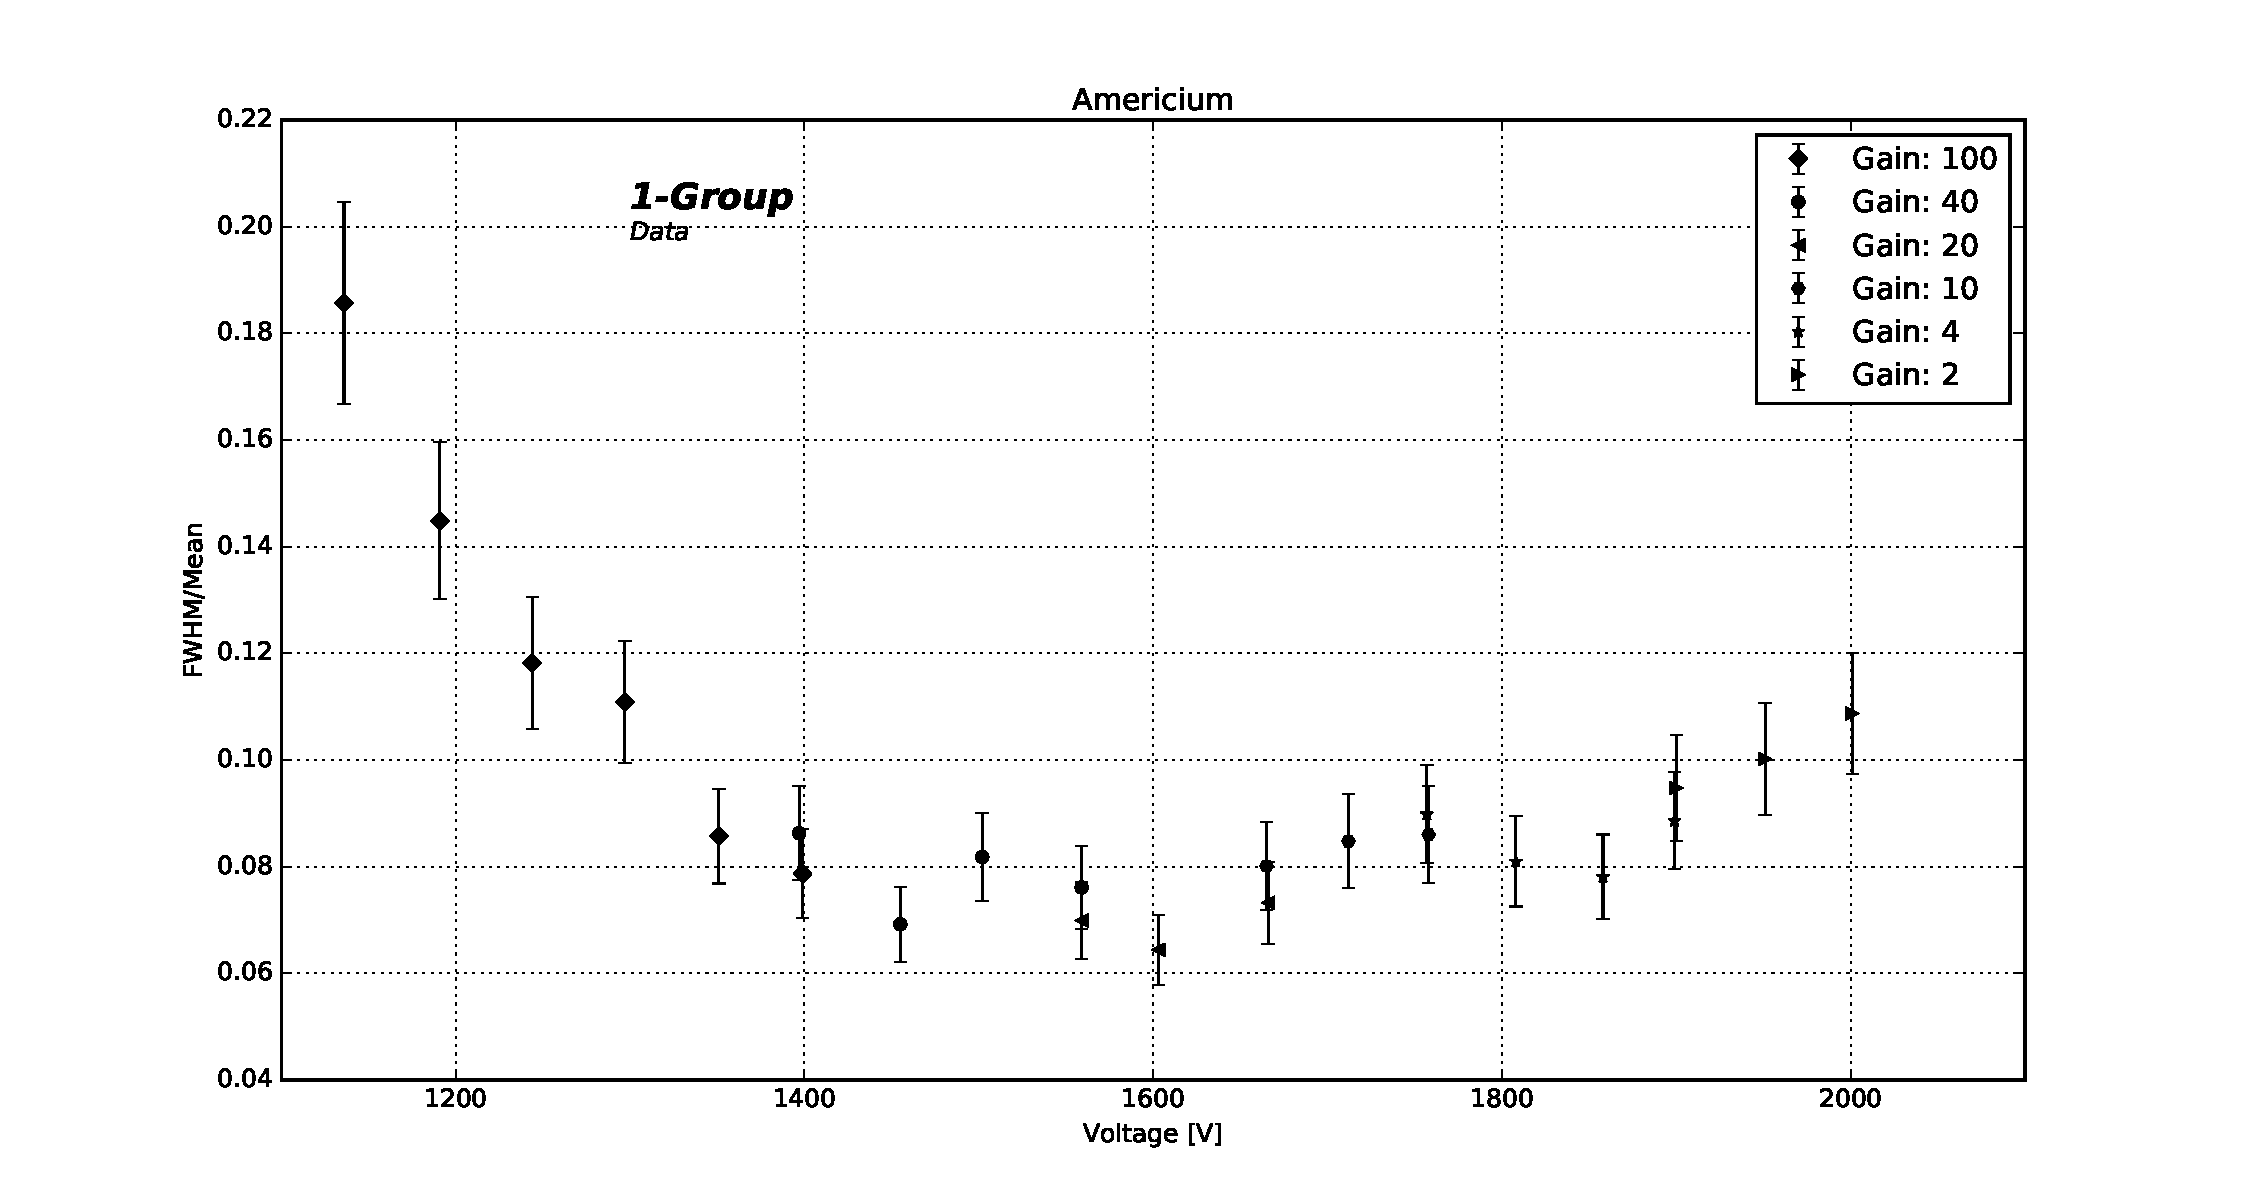
\includegraphics[width=\linewidth]{graphics/americium_scan}
  \caption{Americium scan}
  \label{fig:resolution:americium}
\end{figure}

\begin{figure}[htb]
  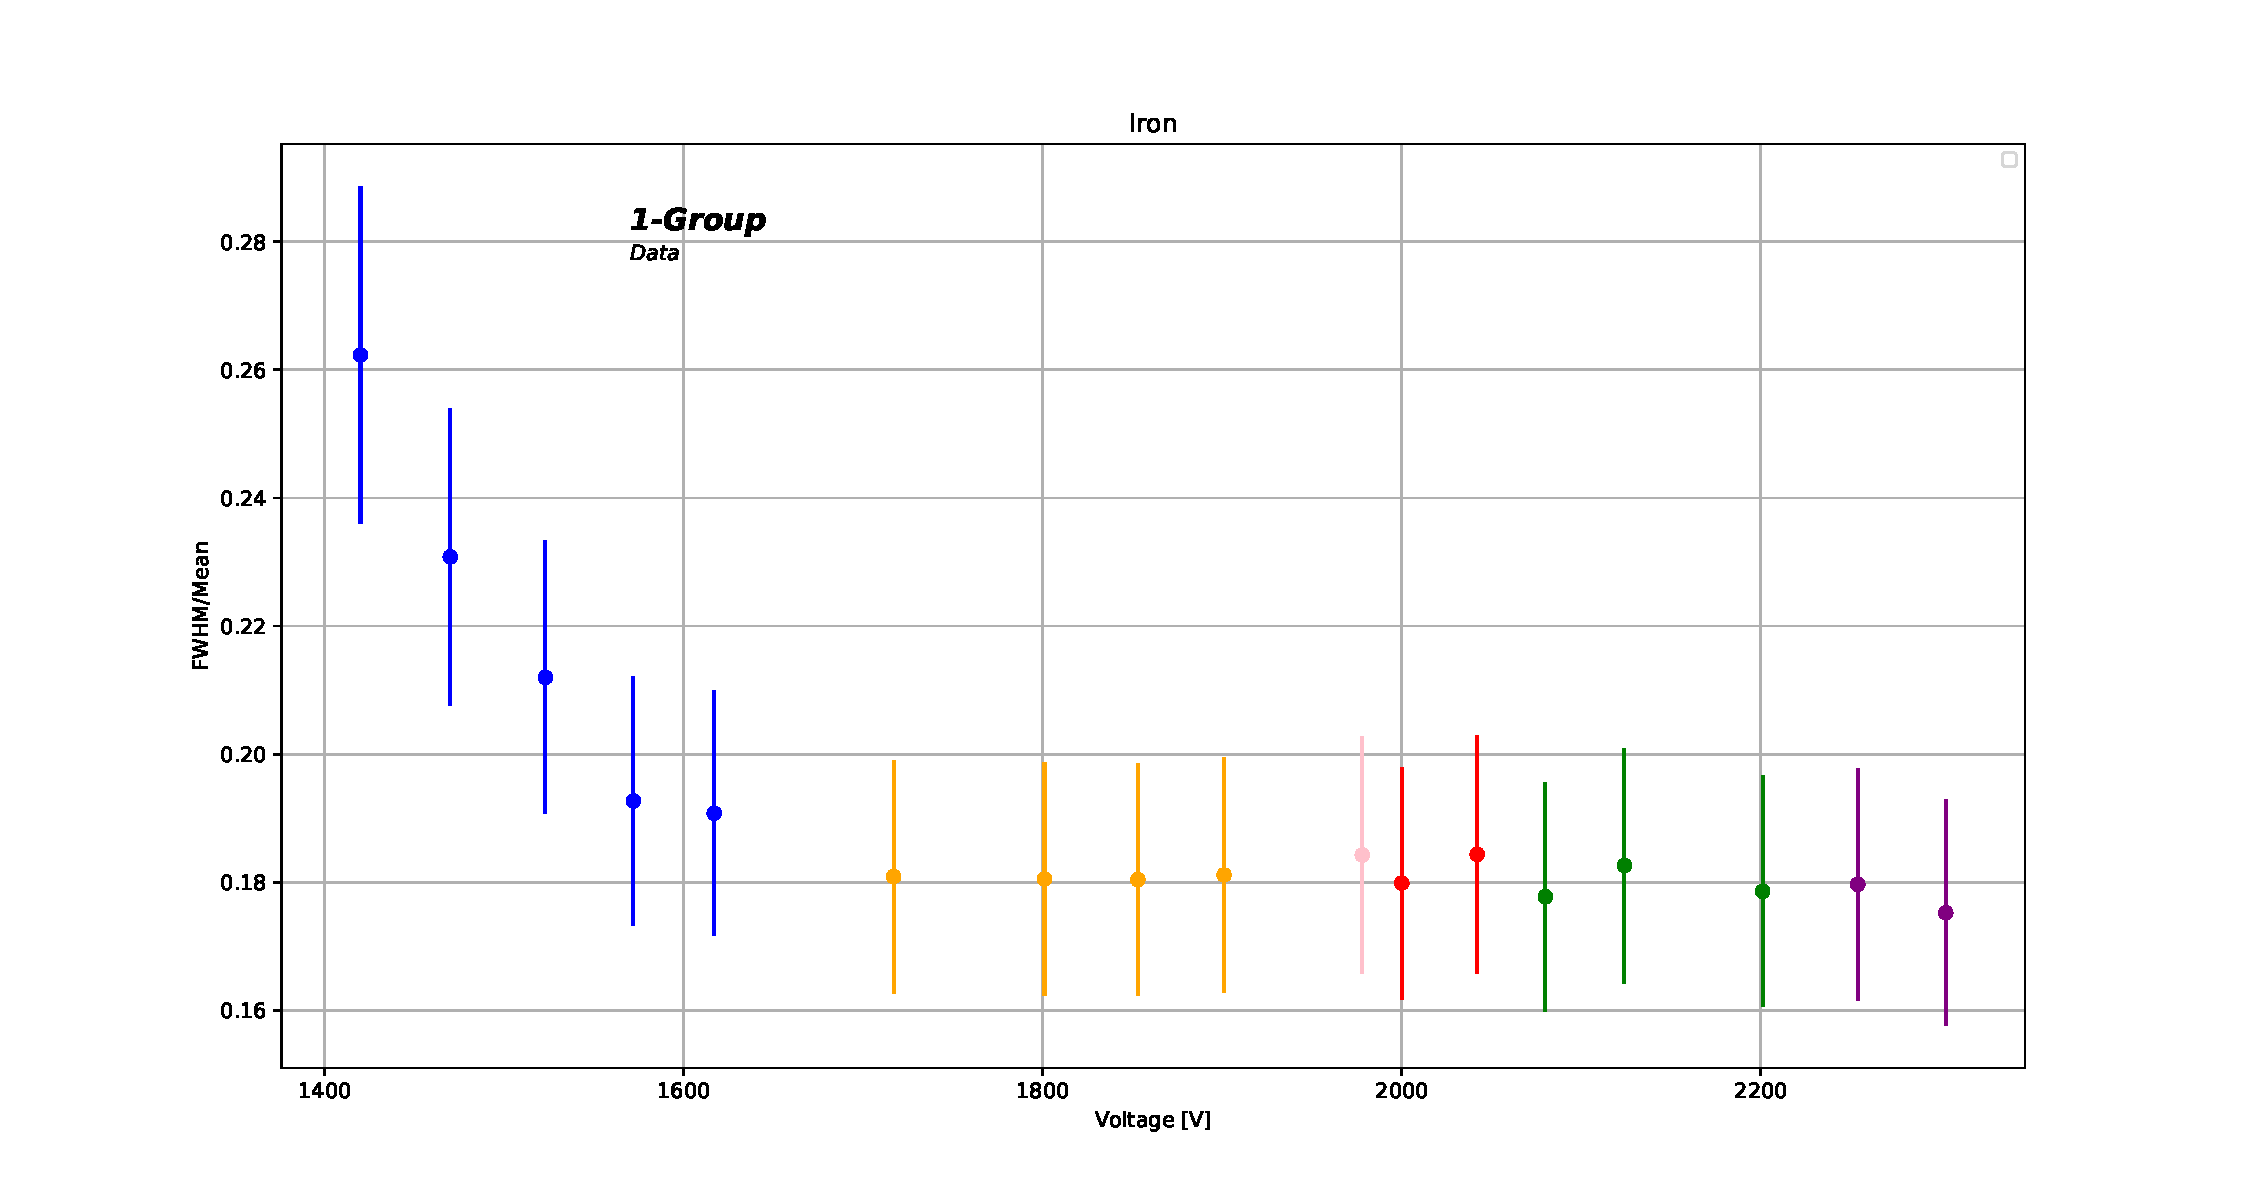
\includegraphics[width=\linewidth]{graphics/iron_scan}
  \caption{Iron scan}
  \label{fig:resolution:iron}
\end{figure}


%%%%%%%%%%%%%%%%%%%%%%%%%%%%%%%%%%%%%%%%%%%%
% Charge multiplication
%%%%%%%%%%%%%%%%%%%%%%%%%%%%%%%%%%%%%%%%%%%%

\section{Charge Multiplication}
\label{sec:systematics}

In Sec.~\ref{sec:energy_scan} the resolution for each voltage (with its coarse gain) is calculated by finding the FWHM and the mean of the characteristic peak of the two materials.
The same data can be used to calculate the collected charge as a function of the applied voltage. In fact, the MCA mean of the peaks can be converted in an amount of charge using the calibration curve in Fig.~\ref{fig:charge_calibration}. Since the data in Figs.~\ref{fig:resolution:americium} and \ref{fig:resolution:iron} are taken at different coarse gains and the calibration data are collected with coarse gain $10$, a factor needs to be applied to correct for the difference, with the factor being $10/G_{coarse}$. For each measurement $i$, then, the collected charge is calculated as such:

\begin{adjustwidth}{-1cm}{}
\begin{align}
Q_{coll, i} = (b + a \cdot mean_{MCA, i}) \cdot \frac{10}{G_{coarse, i}} 
\end{align}
\end{adjustwidth}

where $Q_{coll, i}$ is the collected charge per measurement, $a$ and $b$ are the calibration function parameters from Fig.~\ref{fig:charge_calibration}, $mean_{MCA, i}$ is the mean of the gaussian in the MCA spectrum and $G_{coarse, i}$ is the coarse gain used for the measurement. In order to obtain the number of electrons, $Q_{coll, i}$ is then divided by the charge of one electron $1.602 \cdot 10^{-19}$ C. The results for both Am and Fe are shown in Fig.~\ref{fig:number_of_electrons}, where the errorbars are smaller than the data points. The uncertainties on these points are both statistial and systematics and they are combined in quadrature; in particular, the systematic uncertainties come from the systematic uncertainties on $mean_{MCA, i}$ and on $G_{coarse, i}$.


\begin{figure}[htb]
  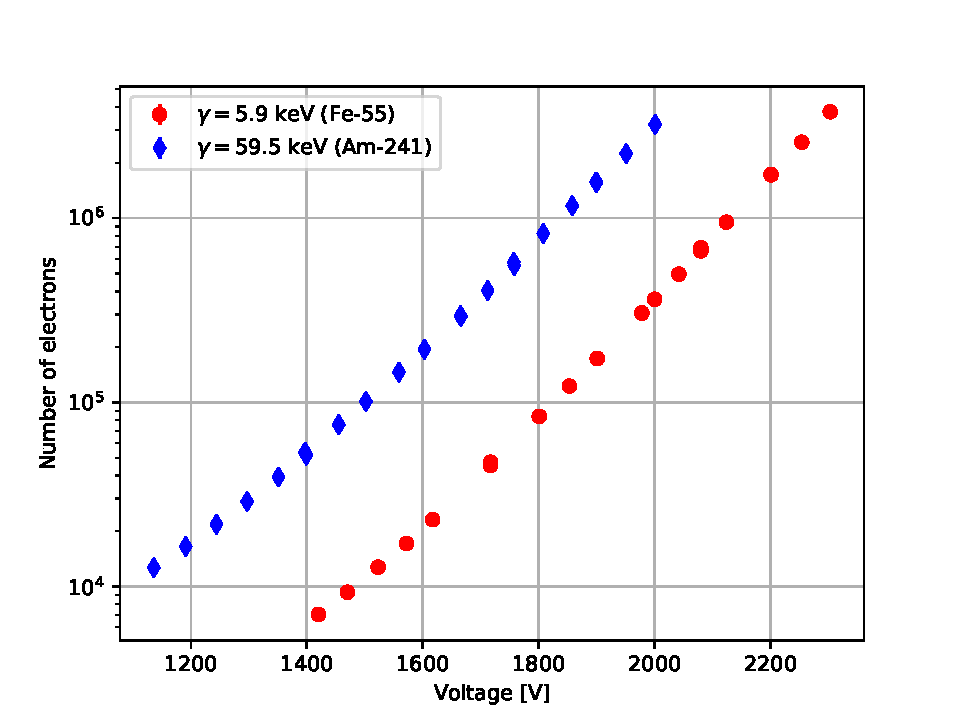
\includegraphics[width=0.5\textwidth]{graphics/numbervsvoltage.pdf}
  \caption{Charge collected in the cider can proportional detector as a function of the voltage applied for the Fe and Am sources. Note that the errorbars are smaller than the plotted points.}
  \label{fig:number_of_electrons}
\end{figure}

After having calculated the number of electrons collected as a function of voltage, we can find the measured multiplication factor per measurement $i$ as

\begin{align}
\label{eq:Mexp}
M_{experimental,i} &= \frac{N_{carriers,out,i}}{N_{carriers per avalanche}} \nonumber \\
                   &= \frac{Q_{coll,i}}{n_{Fe^{5},Am^{241}}\cdot e}
\end{align}

where $M_{experimental,i}$ is the experimentally measured multiplication factor, $Q_{coll,i}$ is the charge collected per measurement, $e$ is the electron charge and $n_{Fe^{55},Am^{241}}$ is the average number of electrons-ion pairs produced by either Fe$^{55}$ (227) or Am$^{241}$ (2290), as taken from \cite{can_paper}.

In order to compare those found values with the theoretical expectation, we computed the multiplication factor with the parameters of our experiment (and of the environment the experiment was conducted in) using this formula, which assumes that our detector is operating in the linear regime (\cite{gas_detect}):

\begin{adjustwidth}{+0.5cm}{}
\begin{align}
\ln(M)=\frac{\ln(2)}{\ln(r_{c}/r_{a})}\cdot\frac{V}{\Delta V}\cdot\ln\left[ \frac{V\rho_{o}}{ra\ln(r_{c}/r_{a})E_{min}(\rho_{o})\rho}\right]
\label{eq:lnm}
\end{align}
\end{adjustwidth}

The meaning and values associated with each parameter of this equation is listed in Tab.~\ref{Tab:params}. One can see that most of these values either come from tabulated properties of the gas used, or are derived from the initial measurement of the beer can dimensions, listed in Tab.~\ref{Tab:cidercan_sizes} for reference.

\begin{table*}[htb]
  \begin{tabularx}{\linewidth}{p{1.5cm}p{8cm}rl}
    \textbf{Variable}     & \textbf{Definition}                                                         & \textbf{Value}     & \textbf{Source}  \\
    \hline
    $r_{c}$                 & radius of the cathode                                                       & $3.121 \pm 0.003$      & Eq.~\ref{eq:rcra}   \\
    &&&\\
    $r_{a}$                 & radius of the anode                                                         & $\SI{25 +- 2}{\micro\meter}$ & Eq.~\ref{eq:rcra}   \\
    &&&\\
    $V$                    & operating voltage                                                           & 1-3 kV             & N/A                \\
    &&&\\
    $\Delta V$             & potential required to produce an additional electron                & $23.6 \pm 5.4$ V   &\cite{gas_detect}   \\
    &&&\\
    $E_{min}(\rho_{o})$      & \begin{tabular}[c]{@{}l@{}}Minimal electric field needed for ionisation\\(at standard pressure)\end{tabular}         & $48. \pm 3$ kV/cm  &\cite{gas_detect}   \\
    &&&\\
    $\rho_{o}/\rho$ & \begin{tabular}[c]{@{}l@{}}Standard density of the gas\\(compared to density at  T=273K and P = 1 bar)\end{tabular}  &                    &Eq.~\ref{eq:gaslaw}, \cite{meteo}\\
    \hline
  \end{tabularx}
  \caption{List of the main systematics sources}
  \label{Tab:params}
\end{table*}

For the geometric properties, the relationship between the measured quantities and the anode radius, is simply $r_{a} = d_{a}/2$, with $d_{a}$ being the radius of the anode wire. Meanwhile, the radii of the cathode is related to the other measurements via Eq.~\ref{eq:rcra}.

\begin{align}
  \label{eq:rcra}
  r_{c} = \frac{D_{outer}}{2}-\tau
\end{align}

where $D_{outer}$ is the outer radius of the cider can and $\tau$ is the can wall thickness.
To determine the gas properties at the environmental conditions of the laboratory, the temperature and pressure of the room need to be measured. With these values on hand, the ratio of gas densities can be determined by using the ideal gas law.

\begin{align}
  \label{eq:gaslaw}
  \frac{\rho}{\rho_{o}} = \frac{P}{P_{o}}\cdot \frac{T_{o}}{T}
\end{align}

with $\rho$ being the gas density, $P$ the gas pressure and $T$ its temperature.
During the measurements, the temperature stayed mostly constant, but the pressure varied over the course of the day, as shown in Fig.~\ref{fig:pressure}. The uncertainty on the pressure was thus selected to be the largest pressure change with respect to standard pressure, over the course of a day.

\begin{figure}[htb]
  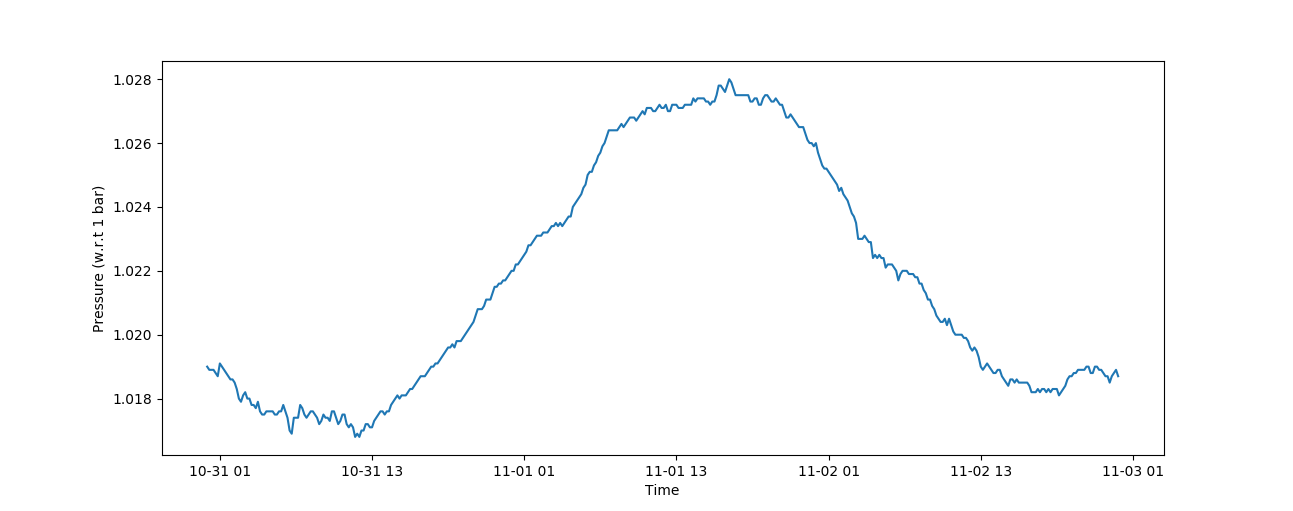
\includegraphics[width=0.5\textwidth]{graphics/pressure_monitoring.png}
  \caption{Atmospheric pressure in Helsinki during the spectra measurement. Source: \cite{meteo}}
  \label{fig:pressure}
\end{figure}

Given the parameters and uncertainties quoted in Tab.~\ref{Tab:params}, a MC simulation was created in order to compute the theoretical uncertainties on the expected multiplication factor as a function of operating voltage. In this systematics treatment, each parameter was drawn out of Gaussian shaped probability distribution, with a mean centred at a parameter's value and the width set as the quoted uncertainty. Fig.~\ref{final_lnm} shows the 1$\sigma$ and 2$\sigma$ confidence interval of the multiplication factor, after propagation of systematic uncertainties.


%The theoretical expectation for the drift chamber's electron yield can be compared to the data obtained during the iron spectrum scan described in Sec.~\ref{sec:resolution_scans}. Given a number of MCA counts $Q_{mca}$, the charge accumulated at the electrodes of the drift chamber can be obtained with Eq.~\ref{eq:M_exp}.

%\begin{align}
%  \label{eq:M_exp}
%  Q_{detector} = \frac{Q_{MCA}}{G_{pre,mca}\cdot{G_{coarse}}}
%\end{align}

%where $G_{pre,mca}$ is the preamplifier gain in units of $d.c./V$ (as plotted in Fig.~\ref{fig:preamp_gain_mca}),and $G_{coarse}$ is the coarse gain that was described and measured in Sec.~\ref{sec:coarse}. From that point, the multiplication factor of the experimental data is given by Eq.~\ref{eq:Mexp}.

%\begin{align}
%  \label{eq:Mexp}
%  M_{experimental} &= \frac{N_{carriers,out}}{N_{carriers per avalanche}} \nonumber \\
%                   &= \frac{Q_{detector}}{n_{Fe^{5},Am^{241}}\cdot e}
%\end{align}

%Where $n_{Fe^{55},Am^{241}}$ is the average number of electrons-ion pairs produced by either Fe$^{55}$ (227) or Am$^{241}$ (2290), as taken from \cite{can_paper}. 

The measured multiplication factors obtained in each voltage scan is shown in Fig.~\ref{final_lnm}, along with the theoretical expectation for their values given the geometry of the can detector and the environmental conditions during the measurement. As one can see, the data collected lies within the $1\sigma$ band of the theoretically predicted values.

\begin{figure}[htb]
  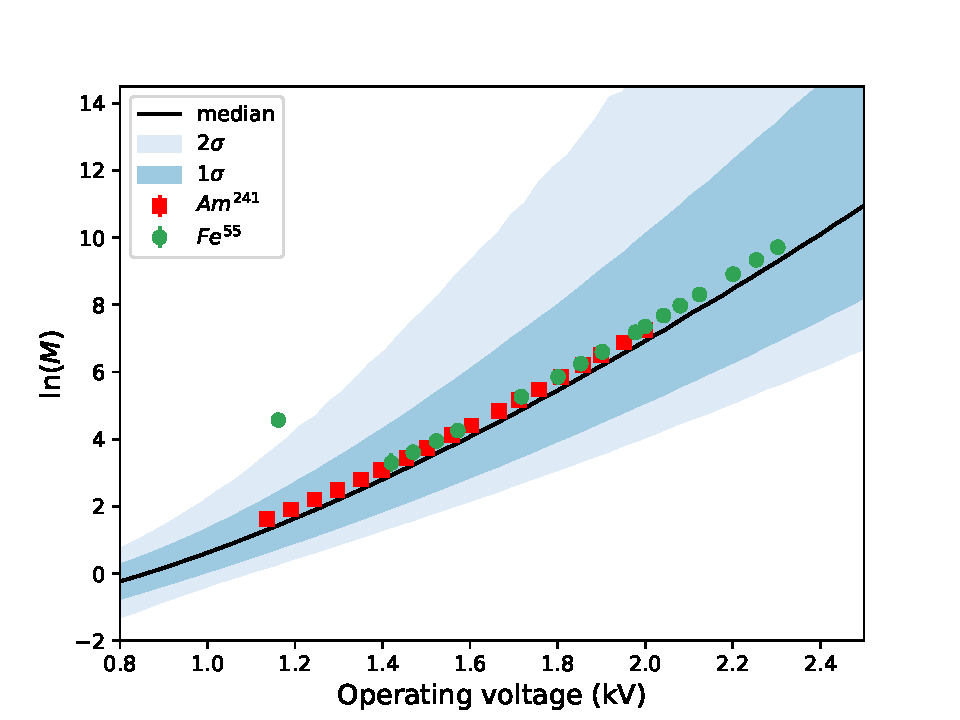
\includegraphics[width=0.5\textwidth]{graphics/lnM_final_plot.pdf}
  \caption{Natural logarithm of the drift chamber's multiplication factor M. Red and green data points represent the results obtained with $Fe^{55}$ and $Am^{241}$ respectively. Blue bands show the theoretical expectation for the detector, given systematics uncertainties in the cider can geometry and gas properties.}
  \label{final_lnm}
\end{figure}
 % Daniel

        \clearpage
	\section{Spectra analysis}
The approximate sweet spot for Am and Fe were rough gain of $4$ and bias voltage of $1937$ V. The measurement times are listed in Tab.~\ref{tab:measurementstimes}. For the can experiment, the sources were collimated.

In this section, the figures for the can and aluminium pipe detectors will be shown side-by-side with the can detector on the left and the aluminium detector on the right.

\begin{table}[hb!]
\begin{tabular}{lll}
\textbf{Detector}    & \textbf{Source} & \textbf{Live time {[}min.{]}} \\ \hline
\multirow{3}{*}{Can} & Fe-55           & 5                          \\
                     & Am-241          & 15                         \\
                     & Bkg             & 45                         \\ \hline
\multirow{3}{*}{Alu} & Fe-55           & 19                         \\
                     & Am-241          & 25                         \\
                     & Bkg             & 30                         \\ \hline
\end{tabular}
\caption{List of measurement times for the different sources and setups.}
\label{tab:measurementstimes}
\end{table}

When the sources are measured, the data files are loaded into histograms which are then converted to cubic basis splines (B-splines) with smoothing of 0.02 for the sources and 0.002 for the background. These are shown as dashed lines in fig. \ref{fig:spectra}. The Am and background spectra are normalized to the Fe spectrum. The splined background is then subtracted from the splined sources and binned into 1024 bits and shown as the full lines in the figure. For the aluminium pipe, the spline procedure does distort the escape peak somewhat. All subsequent figures will only be shown with the background subtracted.

\begin{figure*}[htb]
  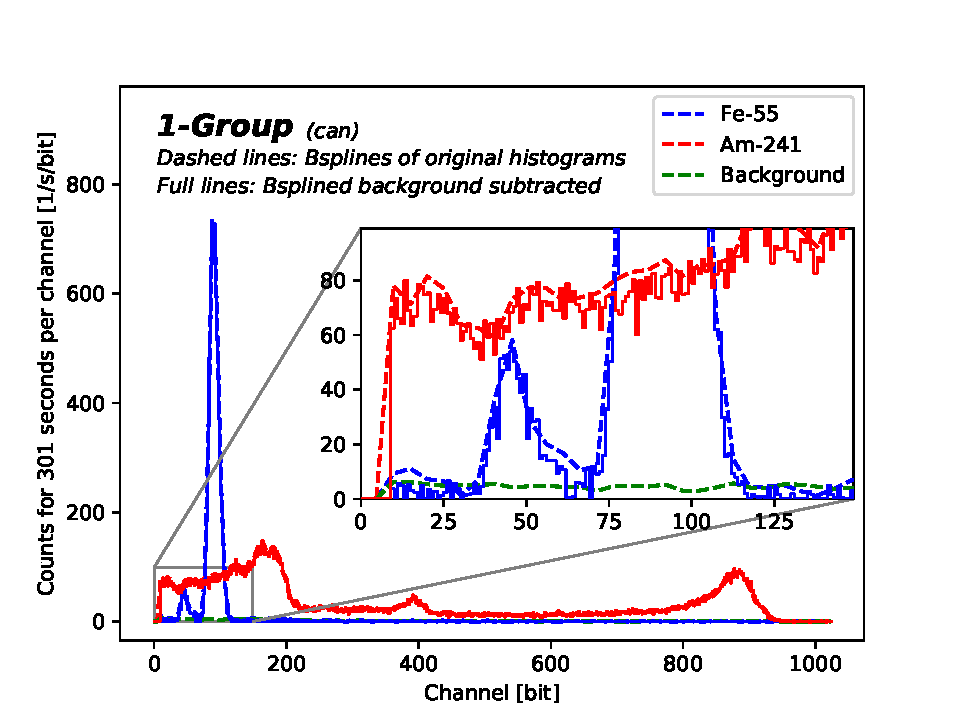
\includegraphics[width=0.49\textwidth,page=1]{graphics/bkgsubtraction.pdf}
  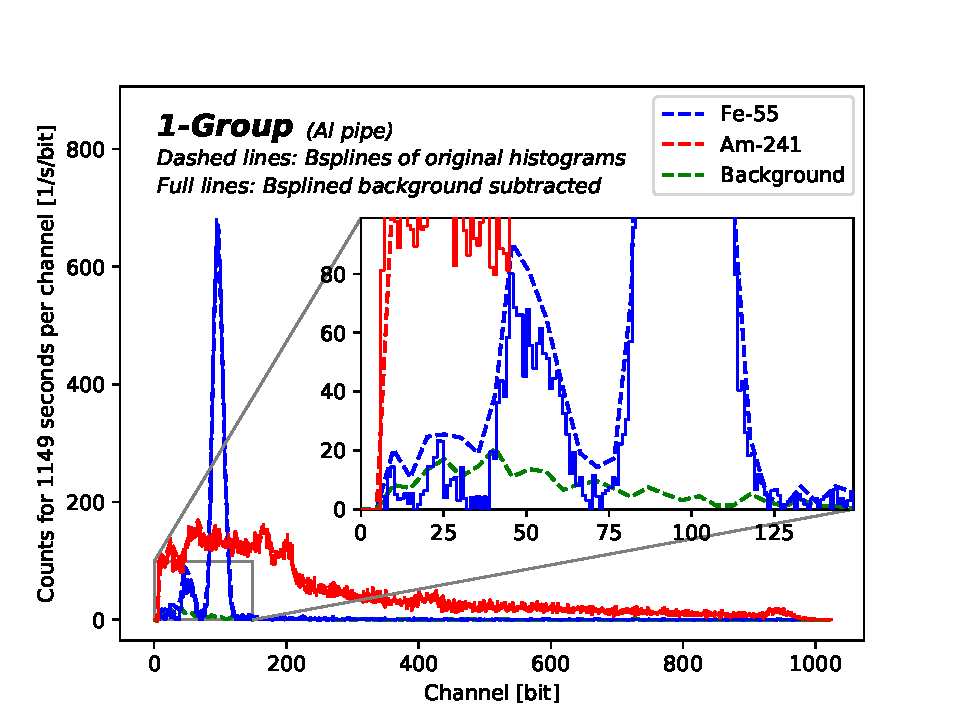
\includegraphics[width=0.49\textwidth,page=1]{graphics/alubkgsubtraction.pdf}
  %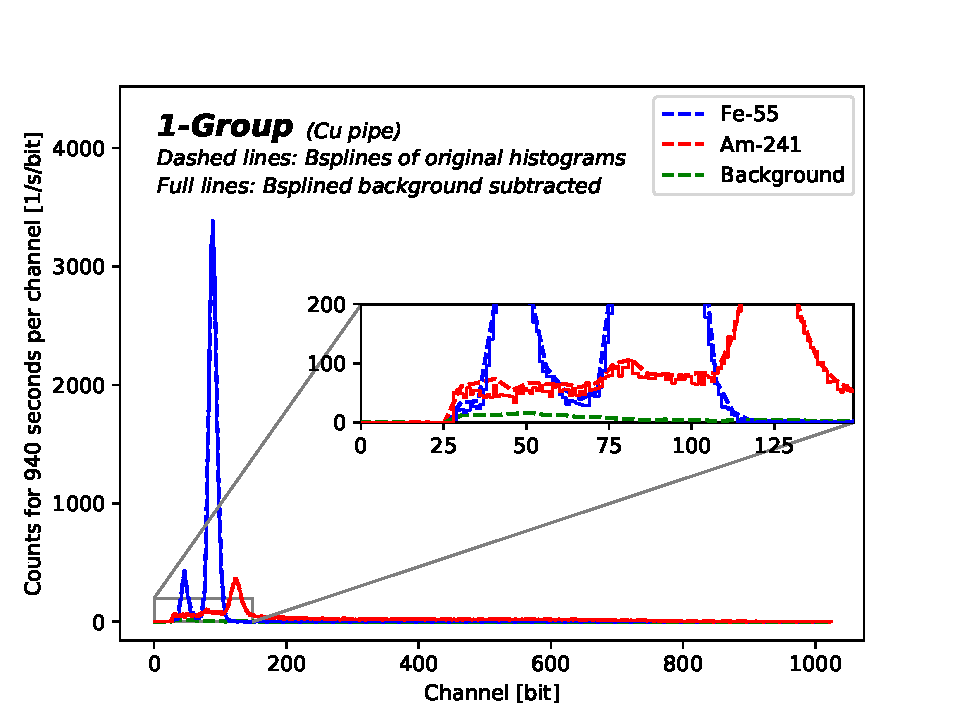
\includegraphics[width=0.32\textwidth,page=1]{graphics/cupbkgsubtraction.pdf}
  \caption{Spectra of Fe and Am as well as background for the can detector and the aluminium pipe. Am and background have been normalized to the Fe spectra. The dashed lines are splines of the original histograms, and the full lines are the splined sources with splined background subtracted. The shown resolution of the splines is intentionally low.}
  \label{fig:spectra}
\end{figure*}

Gaussian fits are then performed on the known Fe and Am peaks. All fits are performed using Chisquare minimization with square root of counts as uncertainties. Different fit functions are used and detailed in table \ref{tab:fitfuncchannelfits}. Fits are first performed with strict bounds which are then entirely lifted to show stability and for correctness of uncertainties. For the can detector, only bins with values larger than 20 are used for the escape peak and the Am peak as chisquare fits with square root uncertainties over-estimate the goodness-of-fit for bins with lows counts. For the Fe double gaussian, the fit spans further in order to reach convergence for the unbounded fit. For the aluminium pipe, the escape peak is badly shaped, possibly due to the spline procedure. Therefore, the fit is performed from the right tail and above the peak until the shape deterioates. For the Fe double gaussian, some of the left side is left out to help convergence of the unbounded fit. For both detectors, the left side of the Am peak is not well modeled by a single gaussian peak, wherefore it is mostly left out from the fit.

For the escape peak fits, a regular gaussian is used. For the Fe peak, the uncorrelated gaussian double gaussian is used. For the Am peak, a regular gaussian is used for the can detector. However, for the aluminium pipe, a 1st order polynomial must be added to ensure convergence.

% \begin{tabular}[c]{@{}l@{}}Uncorrelated\\ double gaussian\end{tabular}
\begin{table*}[htb!]
\begin{tabular}{ll}
\textbf{Name}                 & \textbf{Expression} \\ \hline
Gaussian                      & $\frac{N}{\sqrt{2\pi}\sigma}\exp{\left(-\frac{\left(x-\mu\right)^2}{2\sigma^2}\right)}$                    \\
Uncorrelated double gaussian  & $N\left[r\frac{1}{\sqrt{2\pi}\sigma}\exp{\left(-\frac{\left(x-\mu\right)^2}{2\sigma^2}\right)}+(1-r)\frac{1}{\sqrt{2\pi}\sigma}\exp{\left(-\frac{\left(x-\mu\right)^2}{2\sigma^2}\right)}\right]$                     \\
Gaussian plus 1st order poly. & $\frac{N}{\sqrt{2\pi}\sigma}\exp{\left(-\frac{\left(x-\mu\right)^2}{2\sigma^2}\right)} + b + ax$                   
\end{tabular}
\caption{Expressions for the used fit functions for the gaussian fits. These are regular gaussian functions with a normalization factor. The uncorrelated double gaussian expression is used for fits with overlapping signals, and has less correlated parameters than two regular gaussians. The parameters are the usual gaussian parameters as well as the normalization factor, $N$, the ratio, $r$, and the polynomial factors, the y-intersection, $b$, and the slope $a$.}
\label{tab:fitfuncchannelfits}
\end{table*}

\begin{figure*}[htb]
  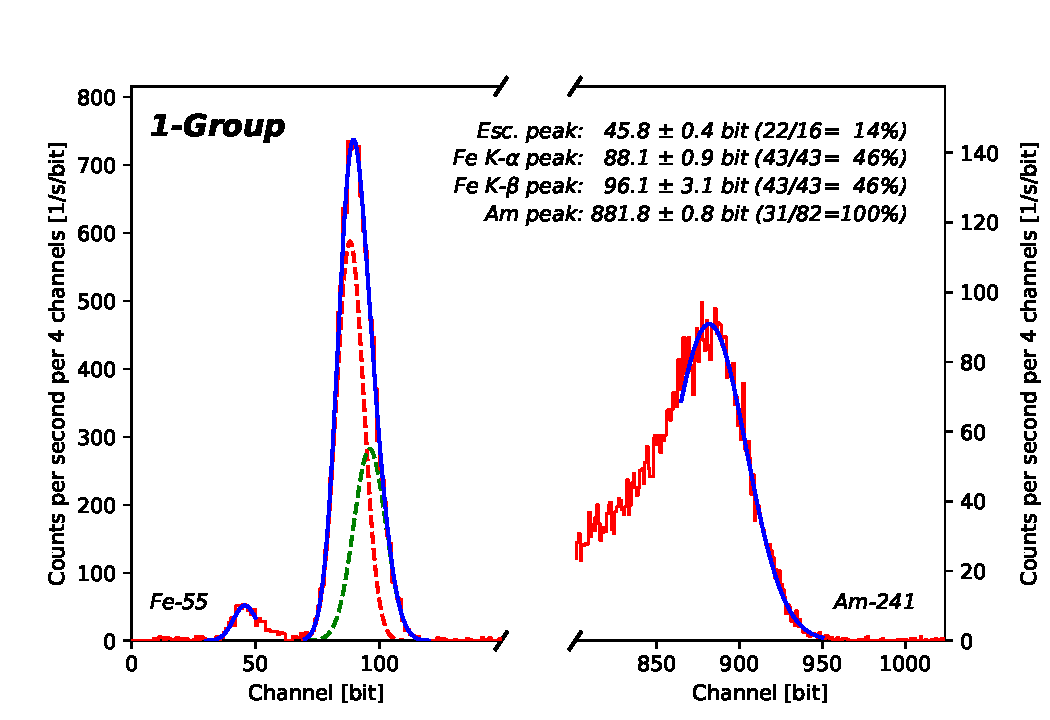
\includegraphics[width=0.49\textwidth,page=1]{graphics/channelfits.pdf}
  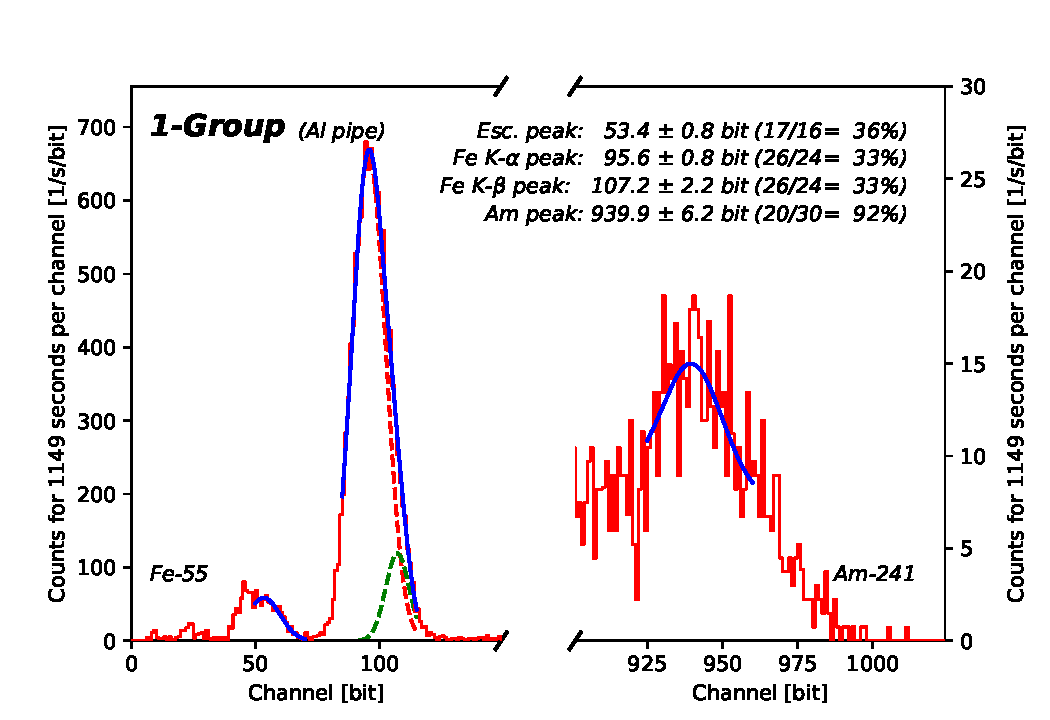
\includegraphics[width=0.49\textwidth,page=1]{graphics/aluchannelfits.pdf}
  \caption{Fits to the four known peaks, the escape peak, the double iron, and the americium. The single gaussians of the double iron peak are shown as dashed lines. The resulting centroids of the fits are shown in the figure along with the Chisquare value, number degrees of freedom, and the Chisquare probability. Note the broken x-axis.}
  \label{fig:channelfits}
\end{figure*}

After extracting the centroids, the four peaks are plotted against their known energies and a 1st order polynomial fit is performed. The result is shown in fig \ref{fig:energychannelcalib}. For the aluminium detector, the low Chisquare value is due to the larger uncertainties coming from the poor gaussian fits, and the y-intersection is not consistent with 0.

\begin{figure*}[htb]
  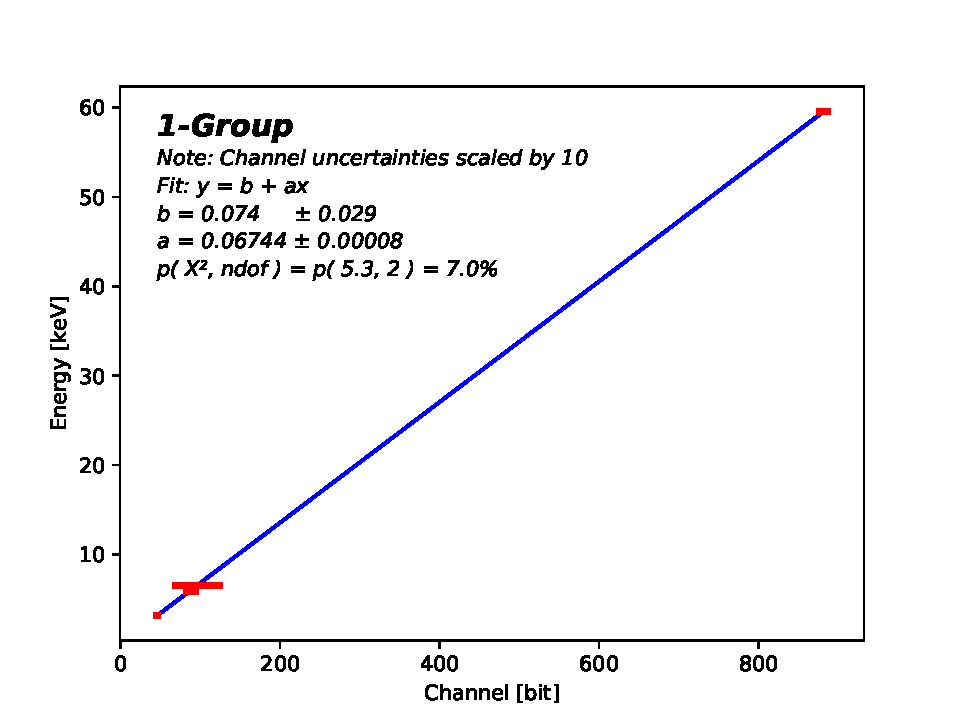
\includegraphics[width=0.49\textwidth,page=1]{graphics/energychannelcalib.pdf}
  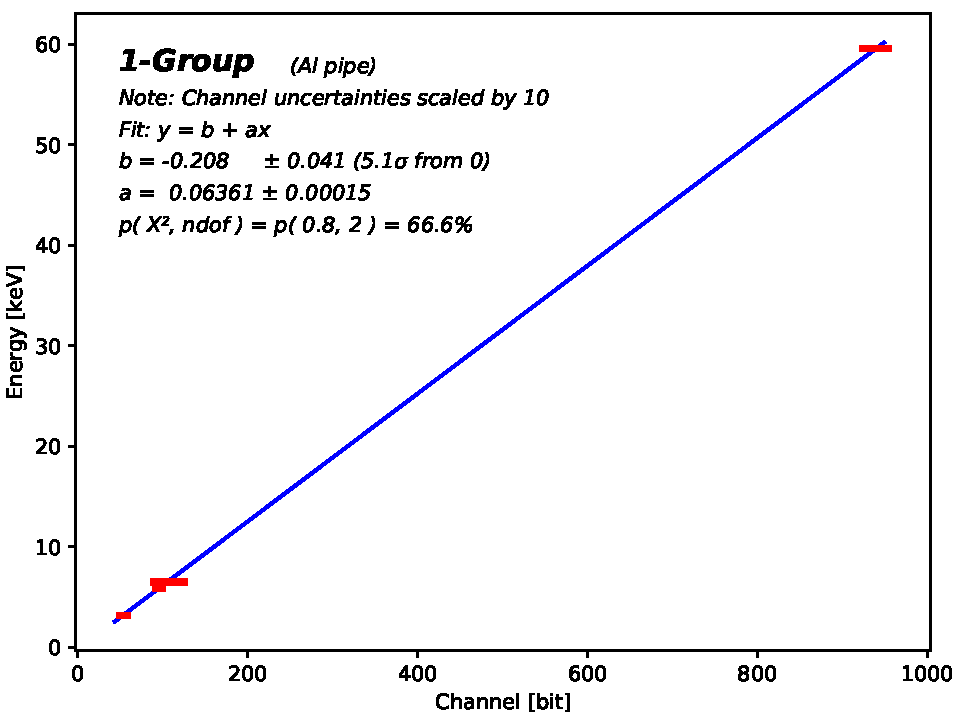
\includegraphics[width=0.49\textwidth,page=1]{graphics/aluenergychannelcalib.pdf}
  \caption{The centroids found in Fig. \ref{fig:channelfits} are plotted against their known energies and fitted with a 1st order polynomial. The y-intersection is not fixed. For the can detector, the uncertainties on the data points are reasonable, while for the aluminium detector, the large uncertainties lead to a smaller Chisquare. For the aluminium detector, the y-intersection is also not consistent with 0. Note that the uncertainties are scaled by 10 to aid visualization.}
  \label{fig:energychannelcalib}
\end{figure*}

With the calibration for conversion of channel to energy, the additional peaks in the americium spectra will be fitted. The result is shown in Fig. \ref{fig:peaksearch}. For the aluminium detector, due to the poor quality, only the biggest of the small peaks were fitted. For this peak, a gaussian with a 1st order polynomial was used, and the same procedure as before was followed.

For the can detector, four peaks were fitted individually with only peak 1 left in a bound fit. All four fits were made with a gaussian plus a 1st order polynomial. Afterwards, all 4 peaks were fit simultaneously with 4 gaussians on a 1st order polynomial background. The starting values used were the gaussian parameters from the previous fits with a $\pm 20\%$ bound. However, the widths of the smaller peaks, 2 and 3, were fixed in the simultaneous fit. The starting values for the polynomial were approximately set with very loose bounds.

In Fig. \ref{fig:peaksearch}, the energy uncertainties of the peaks are shown split into its statistical, calibrational, and systematical components. Tab. \ref{tab:peakschannelenergies} shows the fully combined uncertainties only.

\begin{figure*}[htb]
  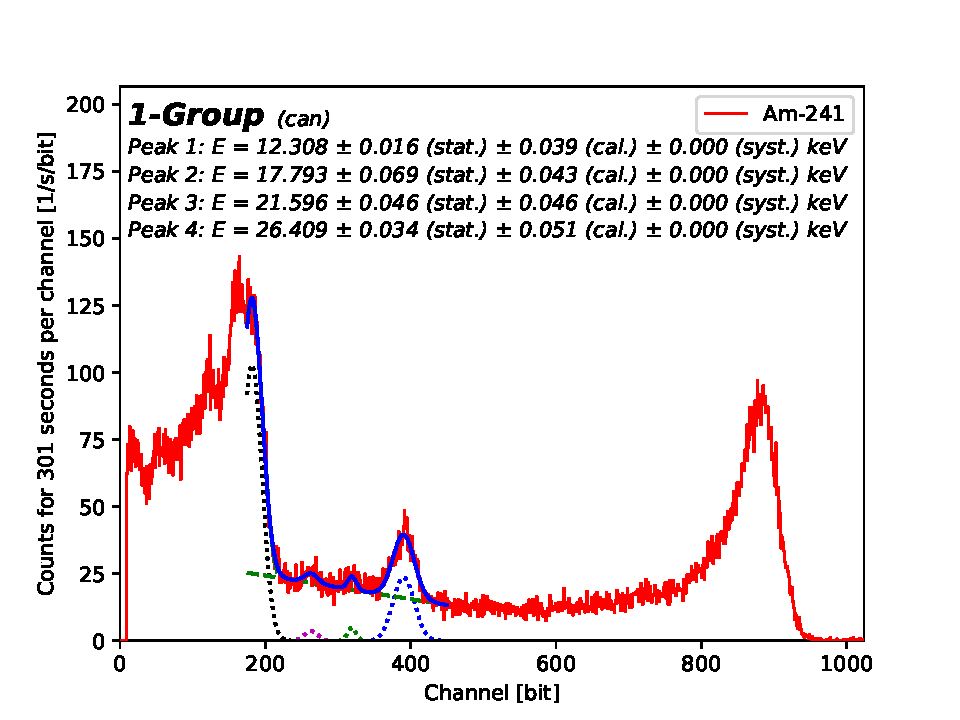
\includegraphics[width=0.49\textwidth,page=1]{graphics/peaksearch.pdf}
  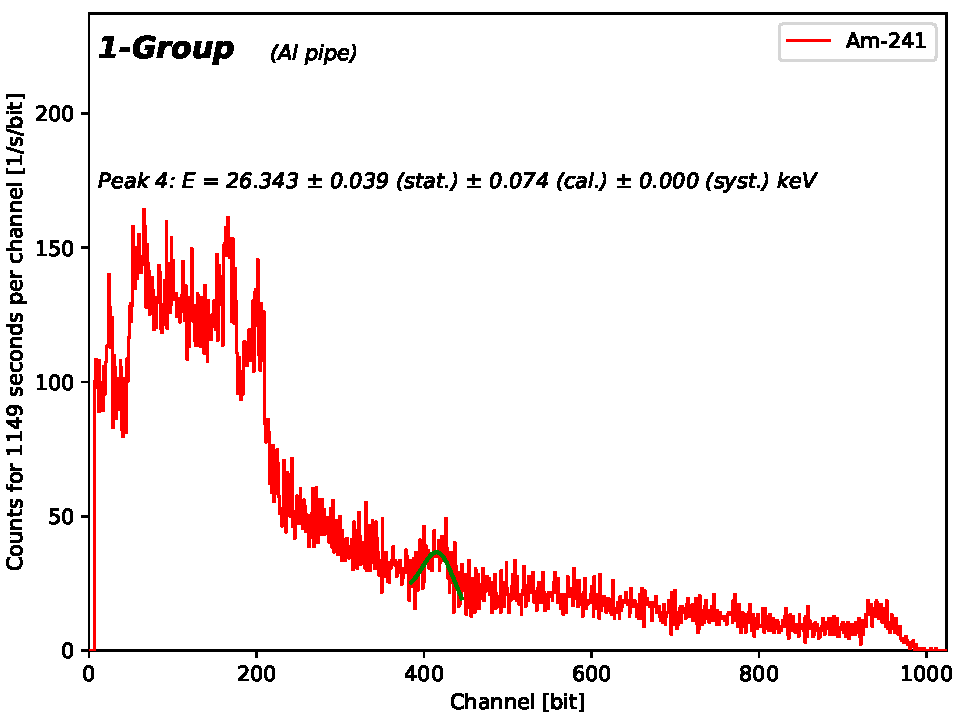
\includegraphics[width=0.49\textwidth,page=1]{graphics/alupeaksearch.pdf}
  \caption{Additional peaks in the americium spectrum are fitted. For the can detector, the individual components of the 4 Gaussians fit are shown in dashed lines. See the text for the fitting details.}
  \label{fig:peaksearch}
\end{figure*}

\begin{table*}[]
\begin{tabular}{lrrrr}
              & \multicolumn{2}{c}{\textbf{Can}} & \multicolumn{2}{c}{\textbf{Alu}} \\
\textbf{Peak} & \textbf{Centroid [bit]}      & \textbf{Energy [keV]}      & \textbf{Centroid [bit]}     & \textbf{Energy [keV]}     \\ \hline
Esc.          & $ 45.90 \pm 0.55$ & $ 3.19$ & $ 53.39 \pm 0.84$ & $ 3.19$ \\
Fe K-$\alpha$ & $ 88.11 \pm 0.91$ & $ 5.89$ & $ 95.64 \pm 0.80$ & $ 5.89$ \\
Fe K-$\beta$  & $ 96.06 \pm 3.13$ & $ 6.49$ & $107.21 \pm 2.22$ & $ 6.49$ \\
Am            & $881.11 \pm 1.06$ & $ 59.5$ & $939.23 \pm 1.92$ & $ 59.5$ \\
1             & $181.58 \pm 0.23$ & $12.31 \pm 0.04$ & - & - \\
2             & $262.82 \pm 1.01$ & $17.79 \pm 0.08$ & - & - \\
3             & $319.16 \pm 0.69$ & $21.60 \pm 0.07$ & - & - \\
4             & $390.45 \pm 0.50$ & $26.41 \pm 0.06$ & $417.38 \pm 0.61$ & $26.34 \pm 0.08$ \\ \hline
\end{tabular}
\caption{List of measurement times for the different sources and setups.}
\label{tab:peakschannelenergies}
\end{table*}

% There's a lot of figures here, and we better flush them out, so they don't mingle way further down the article
\clearpage
         % Daniel

        \clearpage
	\section{Analysis of systematics}
In the analysis of data from experiments, care must be taken to properly take into account systematic uncertainties in our measurements. In the case of the cider can detector, environmental and geometric factors can influence the overall performances of the drift chamber, namely the average number of carriers produced and collected at the electrodes. This number, called the \textit{gain} or \textit{multiplication factor}, can be approximated by the following formula, assuming that our detector is operating in the linear regime(\cite{gas_detect}):

\begin{equation}
  \label{eq:lnm}
  \ln(M)=\frac{\ln(2)}{\ln(r_{c}/r_{a})}\cdot\frac{V}{\Delta V}\cdot\ln\left[ \frac{V\rho_{o}}{ra\ln(r_{c}/r_{a})E_{min}(\rho_{o})\rho}\right]
\end{equation}

The meaning and values associated with each parameter of this equation is listed in table \ref{Tab:params}. One can see that most of these values either come from tabulated properties of the gas used, or are derived from the initial measurement of the beer can dimensions, listed in table \ref{Tab:cidercan_sizes} for reference.

\begin{table}[htb]
  \begin{tabularx}{\linewidth}{X|X|X|p{2cm}}
    \textbf{Parameter}     & \textbf{Definition}                                                         & \textbf{Value}     & \textbf{Source}    \\ \hline
    $r_{c}$                 & radius of the cathode                                                       &                    &\ref{eq:rcra}       \\
    $r_{a}$                 & radius of the anode                                                         &                    &\ref{eq:rcra}       \\
    $V$                    & operating voltage                                                           & 1-3 kV             & N/A                \\
    $\Delta V$             & average potential required to produce an additional electron                & $23.6 \pm 5.4$ V     &\cite{gas_detect}   \\
    $E_{min}(\rho_{o})$      & Minimal electric field needed for ionization (at standard pressure)         & $48. \pm 3$ kV/cm    &\cite{gas_detect}   \\
    $\frac{\rho_{o}}{\rho}$ & Standard density of the gas (compared to density at  T=273K and P = 1 bar)  &                    &\ref{eq:gaslaw} and \cite{meteo} 
  \end{tabularx}
  \caption{List of the main systematics sources}
  \label{Tab:params}
\end{table}

\begin{table}[htb]
  \begin{tabularx}{\linewidth}{X|X|p{2cm}}
    \textbf{Element}                   & \textbf{Measurements}                                 & \textbf{Size}       \\ \hline
    Cider can diameter $D_{outer}$      &                                                       &                     \\
    Cider can wall thickness   $\tau$ & $105 \pm 10 \ \mu$m                                   & $105 \pm 10 \ \mu$m \\
    Plastic tube diameter             & $5.89$ mm, $5.95$ mm, $6.00$ mm, $6.01$ mm, $6.01$ mm &                     \\
    Brass tube diameter               & $1.0$ mm                                              &                     \\
    Nylon screw diameter              & $7.8$ mm, $7.75$ mm                                   &                     \\
    HV connector diameter             & $9.37$ mm                                             &                     \\
    Anode wire diameter               & $50 \pm 10 \ \mu$m                                    & $50 \pm 10 \ \mu$m 
  \end{tabularx}
  \caption{Measurements of the cider can experiment setup components.}
  \label{Tab:cidercan_sizes}
\end{table}

For the geometric properties, the relationship between the measured quantities and the anode radius, is simply $r_{a} = d_{a}/2.$. Meanwhile, the radii of the cathode is related to the other measurements via equation \ref{eq:rcra}.

\begin{equation}
  \label{eq:rcra}
  r_{c} = \frac{D_{outer}}{2}-\tau
\end{equation}

To Determine the gas properties at the environmental conditions of the laboratory, one needed to measure the temperature and pressure of the room. With these values on hand, the ratio of gas densities can be determined by using the ideal gas law.

\begin{equation}
  \label{eq:gaslaw}
  \frac{\rho}{\rho_{o}} = \frac{P}{P_{o}}\cdot \frac{T_{o}}{T}
\end{equation}

During the measurements, the temperature stayed mostly constant, but the pressure varied over the course of the day, as shown in figure \ref{fig:pressure}. The uncertainty on the pressure was thus selected to be the largest pressure change with respect to standard pressure, over the course of a day.

\begin{figure}[htb]
  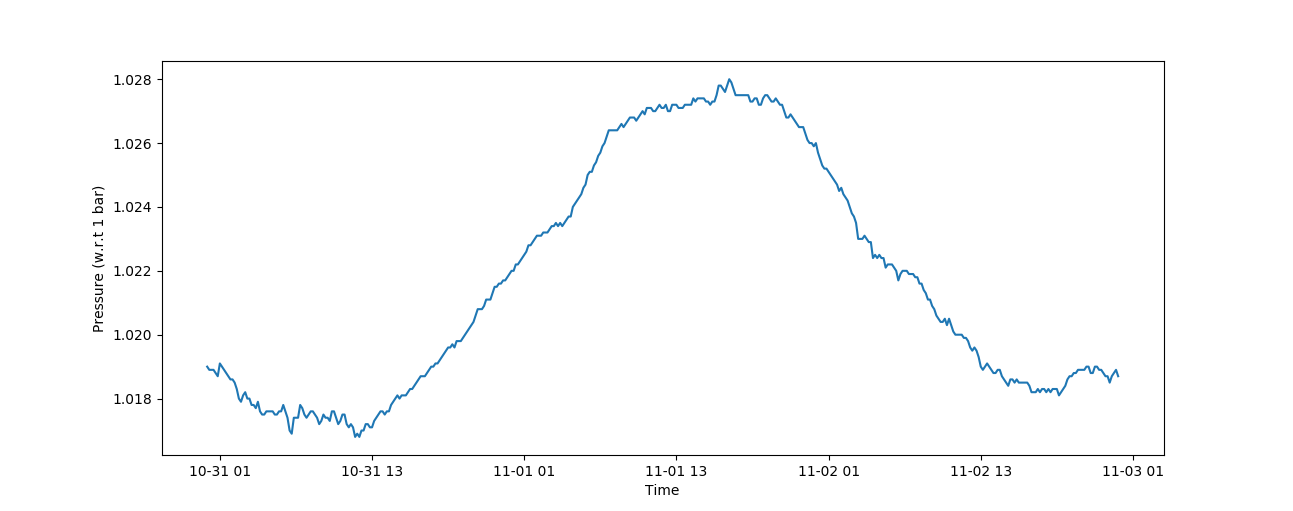
\includegraphics[width=\textwidth]{graphics/pressure_monitoring.png}
  \caption{Atmospheric pressure in Helsinki during the spectra measurement. Source: \cite{meteo}}
  \label{fig:pressure}
\end{figure}

Given the parameters and uncertainties quoted in table \ref{Tab:params}, a MC simulation was created in order to compute the theoretical uncertainties on the expected multiplication factor as a function of operating voltage. In this systematics treatment, each parameter was drawn out of gaussian shaped probability distribution, with a mean centered at a parameter's value and the width set as the quoted uncertainty. Figure \ref{fig:joker_plot} shows the 1$\sigma$ and 2$\sigma$ confidence interval of the multiplication factor, after propagation of systematic uncertainties.

The theoretical expectation for the drift chamber's electron yield can be compared to the data obtained during the iron spectrum scan described in section \ref{sec:voltage_calibration}. Given a number of MCA channels and an output voltage, the charge accumulated at the electrodes of the drift chamber can be obtained with equation \ref{eq:M_exp}.

\begin{equation}
  \label{eq:M_exp}
  Q_{detector} = \frac{V_{output}\cdot c_{preamplifier}}{G}
\end{equation}

where $G$ is the preamplifier gain and its associated uncertainty calculated in section \ref{preampcalib}. From that point, the multiplication factor of the experimental data is given by the following:

\begin{equation}
  M_{experimental} = \frac{Q_{detector}}{n_{Fe^{5}/Am^{241}}\cdot e}
\end{equation}

Where $n_{Fe^{5}/Am^{241}}$ is the average number of electrons-ion pairs produced bu either iron-55 (227) or americium-241 (2290), as taken from \cite{can_paper}.




\begin{table}[]
	\begin{tabularx}{\linewidth}{X|X|p{2cm}}
		\textbf{Element} & \textbf{Measurements} {[}mm{]}                                                  & \textbf{Size} \\ \hline
		Copper tube, length                        & $149.06$, $149.10$, $149.06$, $149.09$                                 &      \\
		Copper tube, wall thickness                & $1.04$, $1.00$, $1.02$, $1.02$, $1.02$, $1.14$, $1.05$, $1.04$, $1.04$ &      \\
		Copper tube, inner radius                  & $19.97$, $19.98$, $19.99$, $19.88$, $19.70$, $19.80$, $19.96$, $20.00$ &      \\
		Copper tube, radiation hole                & $5.03$, $5.04$, $5.08$                                                 &      \\
		Teflon HV front end,  total length         & $36.82$, $36.76$                                                       &      \\
		Teflon HV front end, top part length       & $15.91$, $15.94$, $15.86$                                              &      \\
		Teflon HV front end, tube extremity radius & $19.84$, $19.85$, $19.86$                                              &      \\
		Teflon back end, total length              & $15.04$, $14.97$, $14.89$, $14.93$, $14.95$, $15.06$                   &      \\
		Teflon back end, top part length           & $5.05$, $4.98$, $4.95$                                                 &      \\
		Teflon back end, tube extremity radius     & $19.88$, $19.86$                                                       &      \\
		Brass tube diameter                        & $1.0$                                                                  &      \\
		Anode wire thickened                       & $0.025$                                                                &     
	\end{tabularx}
\caption{Measurements of the copper pipe experiment setup components.}
\label{Tab:coppercan_sizes}
\end{table}
     % Etienne
        
	\clearpage
	\section{Special Detector results}
\label{sec:special_detec}


 % 
	
	\clearpage
	\section{Conclusion}

               % Rosanna
	
	
	
	% === Appendices ======================================================	
	
  \FloatBarrier
	\cleardoublepage
	\appendix
	\section{Resolution scans for Am and Fe}
\label{app:resolution-scans}
  \begin{figure}[htb]
  \foreach \n [count=\i] in {%
    am_100_1136,
    am_100_1191,
    am_100_1244,
    am_100_1297,
    am_100_1351,
    am_100_1399,
    am_40_1397,
    am_40_1455,
    am_40_1502,
    am_40_1559}{
   \begin{subfigure}{.5\linewidth}
        \centering
         \includegraphics[width=\linewidth]{graphics/\n}
        \caption{\detokenize\expandafter{\n}}
      \end{subfigure}
    }
  \end{figure}
  \begin{figure}[htb]\ContinuedFloat
  \foreach \n [count=\i] in {%
    am_20_1559,
    am_20_1603,
    am_20_1666,
    am_10_1665,
    am_10_1712,
    am_10_1758,
    am_4_1757,
    am_4_1808,
    am_4_1858,
    am_4_1899}{
   \begin{subfigure}{.5\linewidth}
        \centering
         \includegraphics[width=\linewidth]{graphics/\n}
        \caption{\detokenize\expandafter{\n}}
      \end{subfigure}
    }
\end{figure}
  \begin{figure}[htb]\ContinuedFloat
  \foreach \n [count=\i] in {%
    am_2_1900,
    am_2_1951,
    am_2_2001} {
   \begin{subfigure}{.5\linewidth}
        \centering
         \includegraphics[width=\linewidth]{graphics/\n}
        \caption{\detokenize\expandafter{\n}}
      \end{subfigure}
    }
    \caption{Scan for different gains and voltages for Americium.}
    \label{fig:scan:americium}
\end{figure}

  \begin{figure}[htb]
  \foreach \n [count=\i] in {%
fe_100_1420,
fe_100_1470,
fe_100_1523,
fe_100_1572,
fe_100_1617,
fe_100_1717,
fe_40_1717,
fe_40_1801,
fe_40_1853,
fe_40_1901}{
   \begin{subfigure}{.5\linewidth}
        \centering
         \includegraphics[width=\linewidth]{graphics/\n}
        \caption{\detokenize\expandafter{\n}}
      \end{subfigure}
    }
  \end{figure}
  \begin{figure}[htb]\ContinuedFloat
  \foreach \n [count=\i] in {%
fe_20_1901,
fe_20_1978,
fe_10_1978,
fe_10_2000,
fe_10_2042,
fe_10_2080,
fe_4_2080,
fe_4_2124,
fe_4_2201}{
   \begin{subfigure}{.5\linewidth}
        \centering
         \includegraphics[width=\linewidth]{graphics/\n}
        \caption{\detokenize\expandafter{\n}}
      \end{subfigure}
    }
\end{figure}
  \begin{figure}[htb]\ContinuedFloat
  \foreach \n [count=\i] in {%
fe_2_2201,
fe_2_2254,
fe_2_2303}{
   \begin{subfigure}{.5\linewidth}
        \centering
         \includegraphics[width=\linewidth]{graphics/\n}
        \caption{\detokenize\expandafter{\n}}
      \end{subfigure}
    }
    \caption{Scan for different gains and voltages for Iron.}
    \label{fig:scan:iron}
  \end{figure}

\FloatBarrier



	
	% === Back matter =====================================================
	
	% References
	%\bibliographystyle{plain}
	%\bibliographystyle{acm}
	\bibliographystyle{unsrt}
	\bibliography{./sections/references}
	\clearpage
	\pagestyle{empty}
	\cleardoublepage
\end{document}
